\documentclass[usenatbib,usegraphicx,letterpaper]{mn2e}
\usepackage[totalwidth=480pt,totalheight=680pt]{geometry}

\usepackage{amssymb}
\usepackage{epsfig}
\usepackage{amsmath}
\usepackage{color}
\usepackage[dvipsnames]{xcolor}
\usepackage{epsfig}  
\usepackage{graphicx}
\usepackage{subfig}
\usepackage{rotating}
\usepackage{array}
%%\usepackage{physics}

%Journals
\def\pasj{{PASJ}}
\def\nat{{ Nature }}
\def\aap{{ Astron. \& Astrophys. }}
\def\aj{{ Astron.~J. }}
\def\apj{{ Astrophys.~J. }}
\def\araa{{ Ann. Rev. Astron. Astrophys. }}
\def\apjl{{ Astrophys.~J.~Letters }}
\def\apjs{{ Astrophys.~J.~Suppl. }}
\def\apss{{ Astrophys.~Space~Sci. }}
\def\icarus{{ Icarus }}
\def\mnras{{ MNRAS }}
\def\pasp{{ Pub. Astron. Soc. Pacific }}
\def\planss{{ Plan. Space Sci. }}
\def\physrep{{ Phys. Rep.}}
\def\jcap{{J. Cosm. Astropart. Phys.}}

% less then similar, greater than similar
\def\lsim{\lower0.6ex\vbox{\hbox{$ \buildrel{\textstyle <}\over{\sim}\ $}}}
\def\gsim{\lower0.6ex\vbox{\hbox{$ \buildrel{\textstyle >}\over{\sim}\ $}}}

% begin equation
\newcommand{\beq}{\begin{equation}}
\newcommand{\eeq}{\end{equation}}
\newcommand{\beqa}{\begin{eqnarray}}
\newcommand{\eeqa}{\end{eqnarray}}

% basic cosmology
\newcommand{\Ho}{H_{0}}
\newcommand{\Om}{\Omega_{\mathrm{M}}}
\newcommand{\Ol}{\Omega_{\Lambda}}
\newcommand{\Ode}{\Omega_{\mathrm{DE}}}
\newcommand{\rhocrit}{\rho_{\mathrm{crit}}}
\newcommand{\Ok}{\Omega_{\mathrm{K}}}
\newcommand{\wzero}{w_{0}}
\newcommand{\wa}{w_{\mathrm{a}}}
\newcommand{\wpiv}{w_{\mathrm{piv}}}
\newcommand{\apiv}{a_{\mathrm{piv}}}
\newcommand{\ellmax}{\ell_{\mathrm{max}}}
\newcommand{\fsky}{f_{\mathrm{sky}}}

\newcommand{\fom}{\mathcal{F}}
\newcommand{\Rvir}{r_{\mathrm{vir}}}
\newcommand{\Rdel}{r_{\Delta}}

% units
\newcommand{\Msun}{\mathrm{M}_{\odot}~}
\newcommand{\hMsun}{\ h^{-1}\mathrm{M}_{\odot}~}
\newcommand{\hMpc}{\ h^{-1}\mathrm{Mpc}~}
\newcommand{\hkpc}{\ h^{-1}\mathrm{kpc}~}
\newcommand{\cpiv}{c_{\mathrm{piv}}}
\newcommand{\kmsmpc}{~\mathrm{km/s/Mpc}~}
\newcommand{\kms}{~\mathrm{km}~\mathrm{s}^{-1}}
\newcommand{\Mpc}{\mathrm{Mpc}}
\newcommand{\kpc}{\mathrm{kpc}}
\newcommand{\pc}{\mathrm{pc}}
\newcommand{\au}{\mathrm{AU}}
\newcommand{\gev}{\mathrm{GeV}}

% roman differential
%\newcommand{\dd}{\mathrm{d}}

% comments
\newcommand{\arz}[1]{{\color{BrickRed}\textbf{[ARZ: }\textbf{#1}]}}


\bibliographystyle{mn2e}

%%%%%%%%%%%%%%%%%%%%%%%%%%%%%%%%%%%%%%%%%%%%%%%%

\begin{document}

\title[Halo Definition and Environmental Effects]{Halo Definition and Environmental Effects}
\author[Villareal et al.]
{Antonio Villarreal$^1$\thanks{E-mail: asv13@pitt.edu},
Andrew R. Zentner$^1$\thanks{E-mail: zentner@pitt.edu}, 
Christopher W. Purcell$^2$\thanks{E-mail: cwpurcell@mail.wvu.edu},\\
 Andrew P. Hearin$^3$\thanks{xxx},
 Frank C. van den Bosch$^4$\thanks{yyy}\\
$^{1}$Department of Physics and Astronomy \& \\
Pittsburgh Particle Physics, Astrophysics, and Cosmology Center (Pitt-PACC),\\ 
University of Pittsburgh, Pittsburgh, PA\\
$^{2}$Department of Physics and Astronomy, \\
West Virginia University, Morgantown, WV}

\date{In preparation}

%%\pagerange{\pageref{firstpage}--\pageref{lastpage}} \pubyear{2015}

%% \label{firstpage}

\maketitle

\begin{abstract}
%% Abstract goes here
Recent work has shown the importance of environment to the properties of dark matter halos. This brings conflict to standard implementations of the halo model and excursion set theory which assume that the properties of a population within the halo is determined by the mass of the halo alone. We seek to find a definition of the size of a halo that allows us to minimize the impact of assembly bias on halo model calculations. We analyze the dependence on environment of our properties using the method of marked correlation functions for several different halo definitions, utilizing the \citet{diemer15} simulations. We find that environmental dependencies are dramatically different as we vary the definition of the halo radius in terms of the overdensity $\Delta$. At large length scales, we find that the majority of assembly bias is removed through suitable redefinition of $\Delta$. We are able to determine that the majority of the reduction in assembly bias is related to the elimination of host halos that would cease to be hosts in catalogs at lower values of $\Delta$. Further, we analyze how different mass cuts affect this methodology. We note that unresolved halos leads to assembly bias being missed and that the most massive halos seem to exhibit minimal assembly bias. We further note that the choice of halo definition can induce assembly bias and consider how this may be interpreted in the context of previous results in the literature.
\end{abstract}

\begin{keywords}
dark matter -- galaxies: halos -- galaxies: formation -- large-scale structure of universe -- methods: numerical
\end{keywords}

%% notes on citation style:
%% \citep{stuff01,stuff02,stuff03} produces (Stuff 2001; Stuff 2002; Stuff 2003)
%% \citet{stuff04} produces "Stuff (2004)" in the main body
%% \\* defines a break in a section title it appears?
%% \begin{enumerate} into \item allows you to do the (i), (ii), (iii) thing 


\arz{We should add Andrew Hearin and Frank van den Bosch. Look into formatting the title correctly. Once I'm happy with the quality of the writing, we'll also need to send this to Benedikt Diemer and Andrey Kravtsov and offer them authorship.}

%-----------------------
\section{Introduction}
\label{section:introduction}
%-----------------------
 \arz{We will need to work on the introduction considerably as we get a better handle on the final results. 
 The first two paragraphs can probably be combined into a single shorter paragraph. I also like to end the first paragraph by telling the reader what it is that we aim to do in the paper. The rest of the introduction will need be be completely rewritten in a more professional manner. However, let's get the middle of the paper complete before we work a lot on the introduction and conclusion sections.
 Please pay close attention to your wording. As an example, it is MUCH preferable to say "galaxies and clusters form within 
 merging dark matter halos" than it is to say "the creation of observed galaxies and clusters is often seen as arising from the 
 hierarchical mergers of dark matter halos." The second option is just too long-winded without adding any information.}

In the current concordance cosmology, the creation of observed galaxies and clusters is often seen as arising from the hierarchical mergers of dark matter halos.\citep{white78}. \arz{Add Blumenthal et al. citation here.} 
Being able to model the properties of dark matter halos and the galaxies within gives us a potential probe for the physical processes that go into galaxy formation. The excursion-set formalism of galaxy clustering \citep{bond91,lacey93,somerville99, zentner06} and the standard halo model of galaxy clustering \citep{seljak00, peacock00, scoccimarro01, berlind02, bullock02, cooray02} both can help us in this task, but rely on underlying asumptions. The first is that the statistics of the objects within a dark matter halo is a function of the mass alone. The second is that the clustering of dark matter halos is a function of mass as well. In this paper we propose a simple redefinition of halo size that will help correct for inaccuracies in these two assumptions.

It has previously been demonstrated that the clustering of halos is dependent on not only the halo mass, but also on the formation time of the halo \citep{sheth04, gao05, wechsler06, croton07, zentner07}. Furthermore, it has been shown that the clustering of a given halo is dependent on the halo concentration \citep{wechsler06}. \arz{Using this twice! argh! Such a sentence is very awkward and unclear. Generally, avoiding using "this" or "that" frequently unless it is absolutely obvious what "this" and "that" are.} This necessitates corrections be made to the standard implementations to account for this. More complicated methodologies have been made to extend to using merger histories directly from simulation \citep{dvorkin11}, as well as to account for the dependence due to concentration \citep{gil11}. The relationship that clustering has to the properties of the halo is commonly referred to assembly bias or environmental effects.

Our method of halo redefinition is motivated by the size of a halo not necessarily being a well-motivated property. What is often referred to as the ``virial radius'' will not contain all gravitational bound dark matter particles in the halo \citep{kazan06}. Rather, it is a matter of convention that does not have a common definition across the literature. For example, some studies have chosen to use halo radius defined with respect to the critical mass density of the universe, while many simulation papers choose to use the mean background mass density of the simulation. Furthermore, the overdensity often used can typically vary from 178 (from basic spherical collapse) to 200 (a common simulation definition) to 337 (``virial'' in $\Lambda\mathrm{CDM}$). This can lead to a change of up to tens of percent in the measured halo radius from one measurement to the other. We choose to define a halo radius in a way that encompasses the nearby environmental effects. These may be due to large scale structure or driven by baryonic physics. Using a simulated box, we can then test how the redefinition of the halo size affects the relationship between the clustering and the properties of the halo. In the case that the properties of the halo become independent of the clustering, it is possible to utilize standard implementations of the halo model without necessitating more complicated theory.
 
In \S~\ref{section:data} of this paper, we discuss the simulated cosmological boxes that we utilize for our statistics and the halo finder utilized. In \S~\ref{section:haloprops}, we consider the properties of interest within our halo simulation and their standard definitions. In \S~\ref{section:methodology}, we discuss the statistics that we have used in order to test for environmental effects and the removal of known mass scaling from these statistics. In \S~\ref{section:results}, we present our results on our tests and consider how each definition affects assembly bias. In \S~\ref{section:conclusions}, we discuss the significance of reducing environmental effects through a redefinition of halo environments and discuss possible applications of our methodology. We also consider the nature of assembly bias as a function of halo definition.

%------------------------------------
\section[]{Simulations and Halo Identification}
\label{section:data}
%------------------------------------

In order to study the effects of halo redefinition, we use three cosmological $N$-body simulations of structure formation. The \citet{diemer15} simulations each utilize a Planck best-fit cosmology with $\Om = 0.32$, $\Ol = 0.68$, and $h_{\mathrm{o}} = 0.67$. We use three simulation boxes with comoving sizes of 125, 250, and 500 $\hMpc$ respectively. The particle masses are $1.6 \times 10^8$, $1.3 \times 10^9$, and $1.0 \times 10^{10} \hMsun$ respectively, implying a total of $1024^3$ particles in each simulation. Furthermore, the three simulations have different force softening scales of $2.4$, $5.8$, and $14 \hkpc$. We refer to each simulation as \simA, \simB, or \simC  \ for the remainder of the paper. This set of simulations allows us to probe the resolution effects inherent in halo finding (due to the varying resolutions of the simulations) and to probe the mass dependence of halo clustering over a wider range of halo masses than would be possible with only one simulation from the set. In particular, \simA~, with its higher resolution, contains the least massive resolved halos, while \simC~has the most robust statistics for the most massive halos as a result of the larger simulation volume.

To identify halos, we use the ROCKSTAR halo finder, which works on the phase space algorithm described in \citet*{behroozi13}. In short, ROCKSTAR determines the initial groupings using a Friends-of-Friends algorithm in phase space before applying the spherical overdensity halo definition in order to determine halo properties of interest. Unbound particles are removed prior to the calculation of halo mass and other halo properties. 

\arz{The following sentences here seem out of place.}
In addition, we take interest of the shape of the halo, which is determined through the sorted eigenvalues of the inertia tensor, with principal ellipsoid axes defined such that $a >b > c$. Some of these parameters are determined after fitting the particles to the Navarro-Frenk-White profile \citet*{nfw97}.

\arz{Try this paragraph again. It is rambling. Also it has structural flaws such as referring to $\Delta$ before defining $\Delta$.} 
While the definition of halo size is fairly straightforward, the individual choices that make up the calculation are not particularly well-motivated. While the virial radius of a halo may be one natural choice, simulations have shown that it often misses gravitationally bound particles \citep*{kazan06}. Halo size has become a matter of definition, with $\Delta=200$ being the most common choice within the literature. However, it is not uncommon to see calculations carried out utilizing $\Delta = 178$, as derived through spherical collapse models, or $\Delta = 337$, as calculated in the case of $\Lambda\mathrm{CDM}$. Given the lack of a well-motivated standard, we choose to redefine the halo in terms of the overdensity parameter, $\Delta$, by defining the halo radius, $\Rdel$, as follows:
\beq
	\bar{\rho}(\Rdel) = \Delta\, \rho_{\mathrm{m}}
\eeq
Here, $\rho_{\mathrm{m}}$ is the mean background mass density of the simulation box, while $\bar{\rho}$ is the mean density within $\Rdel$. It should be noted that the use of the critical density or the mean background mass density is interchanged within the literature. The difference between these two values can be as high as a factor of a few, which will then carry forward into the calculation. We allow the overdensity parameter $\Delta$ to vary over the range of the fiducial definition of $\Delta = 200$ down to values as low as $\Delta = 10$. As discussed above, this change is motivated due to the fact that the definition of halo size is primarily a matter of convention.

%-------------------------------------
\section{Halo Properties}
\label{section:haloprops}
%-------------------------------------

We explore the clustering of halos as a function of a number of halo properties that are commonly explored in the 
literature and can be easily measured for a halo from an individual simulation snapshot. The first of these is the 
halo concentration parameter, 
\beq
c_{\mathrm{NFW}} = \frac{\Rdel}{r_\mathrm{s}},
\eeq
where $\Rdel$ is the radius of the halo given an overdensity parameter $\Delta$ used to define the halo and 
$r_{\mathrm{s}}$ is the halo scale radius. \arz{The scale radius has not yet been defined. How will 
the reader know what it is? How is it computed? You should probable introduce the NFW profile here 
rather than above (see my earlier comment on that).}
We also use an additional measure of the concentration of the halo density profile, 
\beq
c_{\mathrm{V}} = \frac{V_{\mathrm{max}}}{V_{\Delta}}, 
\eeq
where $V_{\mathrm{max}}$ is the maximum circular velocity achieved within the halo and $V_{\Delta}$ is the circular 
velocity at the halo radius, $\Rdel$. The quantity $c_{\mathrm{V}}$ can be measured from simulations without 
any need for fitting halo density profiles to determine scale radii and is therefore robust to choices of halo profiles 
and fitting methods. 

Halo concentrations are useful to explore for these purposes for a number of reasons. First of all, environment dependence 
of concentrations is of direct interest in modeling galaxy clustering and gravitational lensing statistics. Secondly, 
concentrations can be measured 
from individual simulation snapshots relatively easily yet halo concentrations are known to be strongly correlated with the formation 
histories of dark matter halos with earlier forming halos having higher concentrations at fixed halo mass 
\arz{Cite papers here like Wechsler et al. 2002}. As such, exploring the concentration dependence of halo clustering may 
yield insight into the age dependence of halo clustering without the need for constructing merger trees. This 
is particularly important in the present study in which the halo finding is performed repeatedly and constructing a 
merger tree for each run of the halo finder with different $\Delta$ can be prohibitive. We will explore measures of 
halo age directly in a forthcoming follow-up study dedicated to halo formation histories.


Figure~\ref{fig:cnfwrelation} shows the mean $c_{\mathrm{NFW}}$-$M_{\Delta}$ relation for halos defined with $\Delta=200$ 
in \simA, \simB, and \simC. For each simulation, we consider halos only above a minimum mass, as shown in Fig.~\ref{fig:cnfwrelation}, to ensure that concentration measurements are not compromised by resolution. Likewise, Figure~\ref{fig:cvrelation} shows the analogous 
relation for the alternative definition of halo concentration, $c_{\mathrm{V}}$. 

%------------------------------------------ Figure for Cnfw(M)
\begin{figure}
\centering
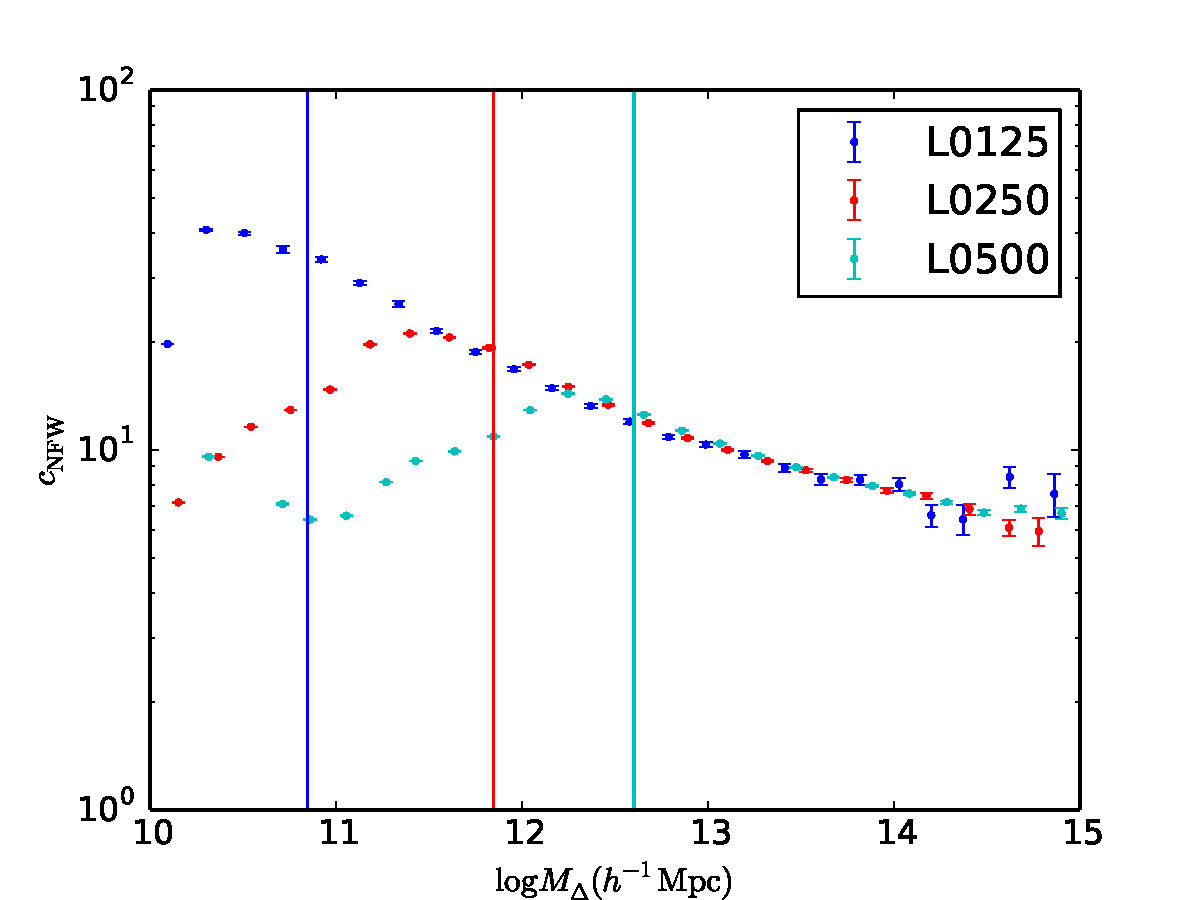
\includegraphics[width=.5\textwidth]{masscut_cnfw_d200.pdf}
\caption{An example of the relationship between the NFW concentration and halo mass for each of our simulations for $\Delta =200$. The chosen lower limit on halo mass for our sample is marked as a blue, red, or cyan line for \simA, \simB, and \simC \ respectively. At lower mass, halos are likely ill defined due to resolution limits.}
\label{fig:cnfwrelation}
\end{figure}
%--------------------------------------------------------------------------------


%------------------------------------------ Figure for C_V(M)
\begin{figure}
\centering
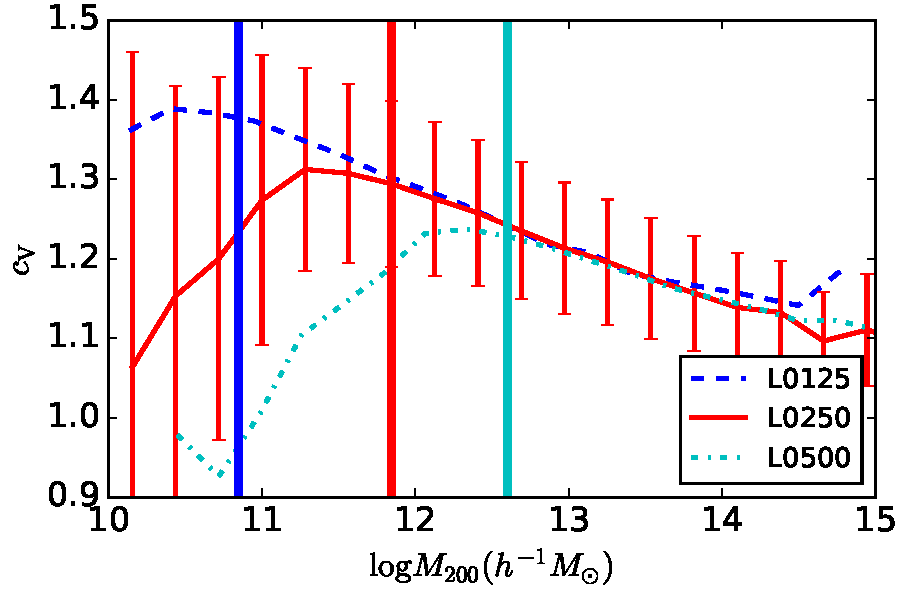
\includegraphics[width=.5\textwidth]{masscut_cV_d200.pdf}
\caption{An example of the relationship between the velocity ratio concentration and halo mass for each of our simulations for $\Delta =200$. The chosen lower limit on halo mass for our sample is marked as a blue, red, or cyan line for \simA, \simB, and \simC \ respectively. At lower mass, halos are likely ill defined due to resolution limits.}
\label{fig:cvrelation}
\end{figure}
%--------------------------------------------------------------------------------

Figure~\ref{fig:concentrations} shows the relationship between $c_{\mathrm{NFW}}$ and $c_{\mathrm{V}}$ for quantifying halo 
concentration on a halo-by-halo basis. Generally the two proxies for concentration are related to each other in a simple manner 
with relatively small scatter indicating that these two quantities largely contain the same information about each halo.

%-------------------------------------------- Figure comparing Cnfw and Cv on a halo-by-halo basis
\begin{figure}
\centering
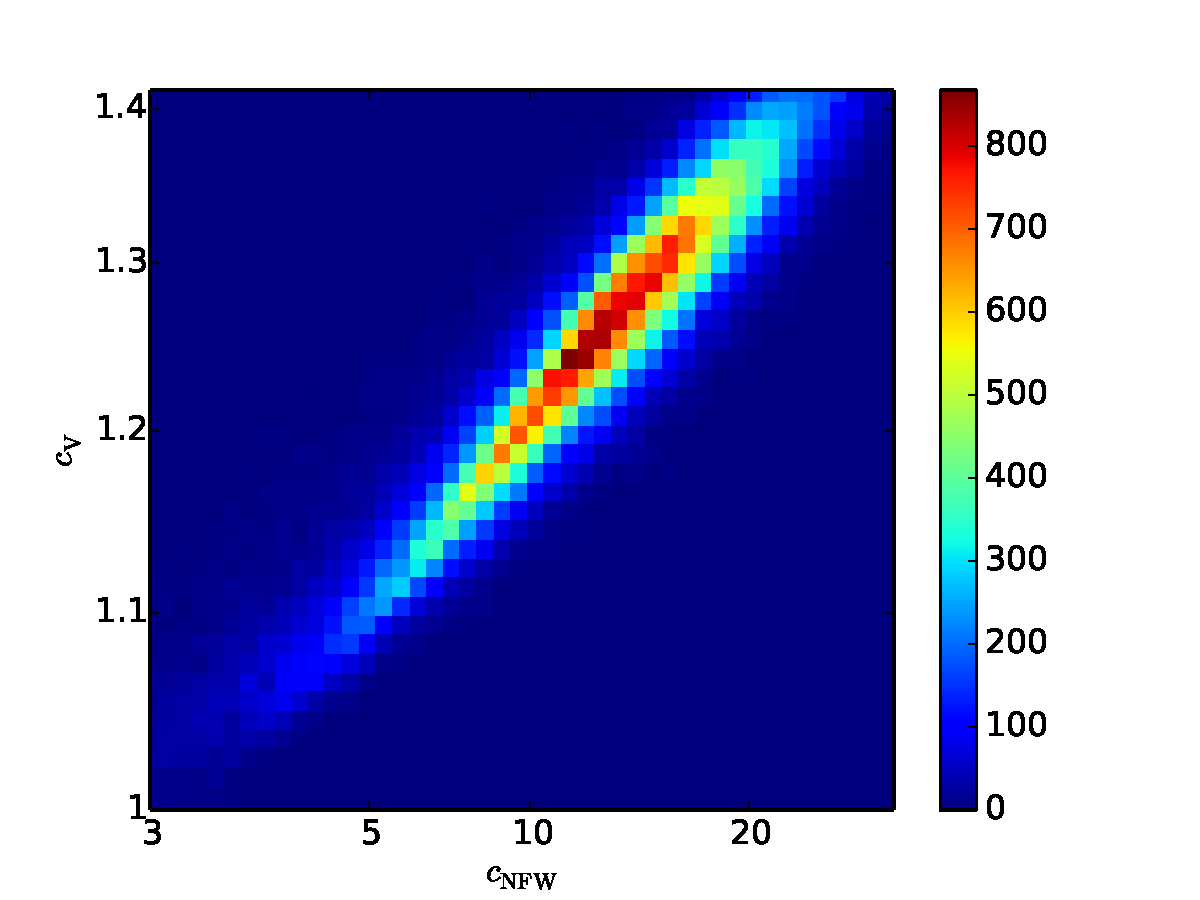
\includegraphics[width=.5\textwidth]{L0250_compare_cnfwvcV_z00.pdf}
\caption{The relationship between the two different marks of concentration, using halos in \simB. 
\arz{This is not sufficiently specific as a caption. For example, you don't say what the color code is 
or what the color scale is.}}
\label{fig:concentrations}
\end{figure}
%--------------------------------------------------------------------------------------------------------------------------------

In addition to halo concentrations, we explore halo clustering as a function of a variety of other 
halo properties. We explore halo clustering as a function of halo shape quantified by the ratio of 
the minor and major axes length, 
\beq
s = \frac{c}{a},
\eeq
where $a$ is the major axis length and $c$ is the minor axis length. The mean relations of halo shapes 
as a function of halo mass for $\Delta=200$ is shown in Figure~\ref{fig:srelation} along with the mass 
thresholds selected to ensure that our results are not compromised by resolution.


%------------------------------------------ Figure for s(M)
\begin{figure}
\centering
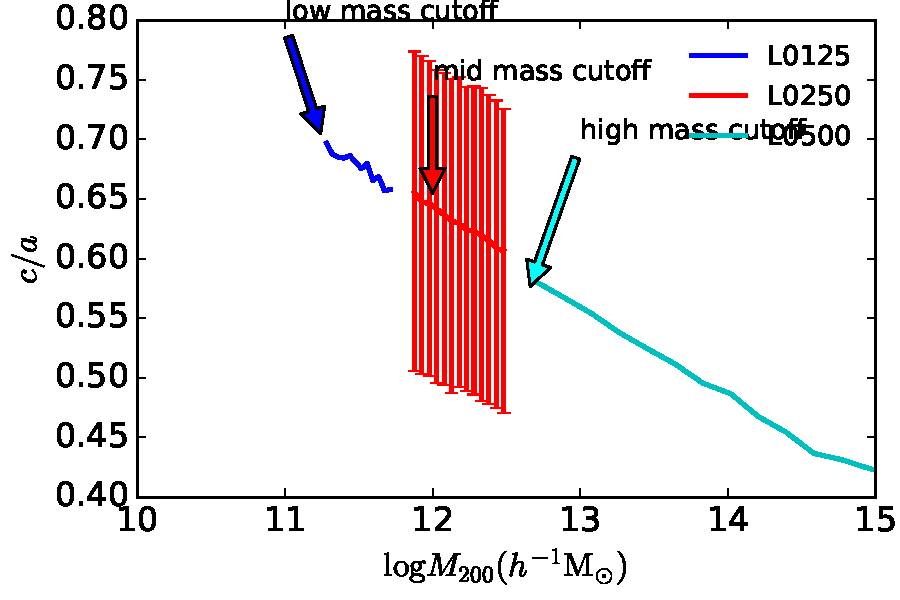
\includegraphics[width=.5\textwidth]{masscut_shape_d200.pdf}
\caption{An example of the relationship between halo shape and halo mass for each of our simulations for $\Delta =200$. The chosen lower limit on halo mass for our sample is marked as a blue, red, or cyan line for \simA, \simB, and \simC \ respectively. At lower mass, halos are likely ill defined due to resolution limits.}
\label{fig:srelation}
\end{figure}
%--------------------------------------------------------------------------------

We also explore halo clustering as a function of halo spin quantified by the spin parameter $\lambda$ as introduced by \citep{peebles69},
\beq
\lambda = \frac{J \sqrt{\lvert E\rvert}}{G M_{\Delta}^{2.5}}
\eeq
where $J$ is the halo angular momentum, $E$ is the total energy of the halo, and $M_{\Delta}$ is the mass at the halo radius, $r_{\Delta}$. The mean relations of halo spins as a function of halo mas for $\Delta=200$ is shown in Figure~\ref{fig:spinrelation} along with the mass thresholds selected to ensure that our results are not compromised by resolution.

%------------------------------------------ Figure for lambda(M)
\begin{figure}
\centering
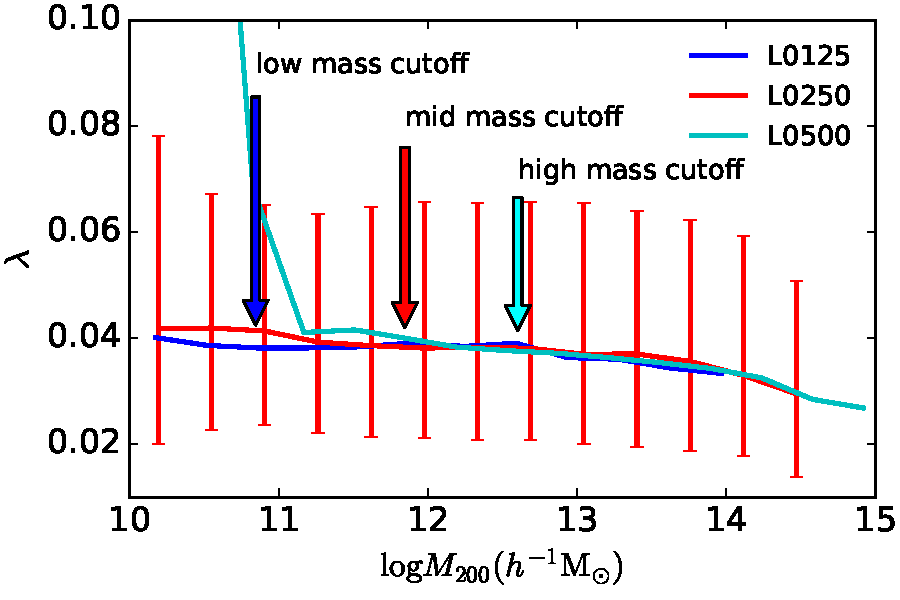
\includegraphics[width=.5\textwidth]{masscut_spin_d200.pdf}
\caption{An example of the relationship between halo spin $\lambda$ and halo mass for each of our simulations for $\Delta =200$. The chosen lower limit on halo mass for our sample is marked as a blue, red, or cyan line for \simA, \simB, and \simC \ respectively. At lower mass, halos are likely ill defined due to resolution limits.}
\label{fig:spinrelation}
\end{figure}
%--------------------------------------------------------------------------------

In practice, the mean relations between the various halo properties and the mass thresholds must be determined 
for each combination of simulation, halo property (e.g., $c_{\mathrm{NFW}}$ or $s$), and halo definition (e.g., value 
of $\Delta$). We use thresholds determined by the particular case under consideration so as to ensure that resolution 
limitations do not drive any of our primary results. A higher mass threshold necessarily means that we do not have any issues due to halo resolution, but reduces the statistics. In addition, it should be noted that halo assembly bias is weakest in the most massive halos, which may reduce the potential signal at high masses. As an example, we summarize some of the mass thresholds we have 
used for a set of $\Delta$ values in Table~\ref{table:thresholds}.

%%%%%%%%%%%%%%%%%%%%%%%%%%%%%%%%%%%%%%%%%%%%%%%%%%%%%%%%%%%%%%%%%%%%%%%%%%%%
\begin{table*}
\caption{
Minimum mass thresholds for each of our analyses depending upon the value of the overdensity, $\Delta$, used to define the halos. In the columns below the values of $\Delta$ we show the minimum host halo masses considered in units of $h^{-1}\mathrm{M}_{\odot}$.}
\vspace*{8pt}
\begin{tabular}{ c c c c c }
\hline
\hline
Cutoff Name \ \  & $\Delta=200$ & $\Delta=100$ & $\Delta=75$ & $\Delta=50$ \\
\hline
\\{low mass} & $7 \times 10^{10}$ & $8 \times 10^{10}$ & $9 \times 10^{10}$ & $1 \times 10^{11}$  \\
{mid mass} & $7 \times 10^{11}$ & $8 \times 10^{11}$ & $9 \times 10^{11}$ & $1.5 \times 10^{12}$ \\
{high mass} & $4 \times 10^{12}$ & $5 \times 10^{12}$ & $6 \times 10^{12}$ & $7 \times 10^{12}$ \\
\hline
\hline
\end{tabular}
\label{table:thresholds}
\end{table*}
%%%%%%%%%%%%%%%%%%%%%%%%%%%%%%%%%%%%%%%%%%%%%%%%%%%%%%%%%%%%%%%%%%%%%%


%-----------------------
\section[]{Methodology}
\label{section:methodology}
%-----------------------

There are several well understood effects in our simulation that must be accounted for before we can draw any conclusions. The first is the matter of simulation resolution. In each of our generated halo catalogs, we can anticipate finding artificial halos. While existing under our constraint of having only a set overdensity, they will have properties that conflict with well known trends that have been shown in prior works, such as concentration decreasing as a function of halo mass \citep{wechsler06}. As shown in Figure~\ref{fig:cnfwrelation}, we can roughly identify the region in which these artificial halos become significant by determining where the monotonic relationship between concentration and mass breaks at low mass. In order to avoid our halo finding statistics being thrown off by these artificial halos, we set a lower mass threshold, limiting the sample to only those halos that are physically significant. We have chosen our threshold to be set by \simB \ in order to minimize the shift to the remaining catalogs.

Another well known effect is the scaling of our properties as a function of halo mass, as well demonstrated within the literature \citep{duffy08}. We are interested in the clustering behavior beyond this well known effect, so we seek to remove this scaling. We take all host halos of interest and sort them by their halo mass. Each set of halo properties are then placed in bins of equal population in order to assure that enough data points exist for robust statistics. We then normalize each mark in a given bin to the mean value. The end result is halo properties that do not change as a function of mass, allowing us to more accurately analyze clustering behavior within our simulation.

To normalize the satellite number we follow the prescription of \citet{wechsler06}. In addition to the mass cutoffs on our data, we eliminate ill-resolved satellites by choosing a cutoff in $v_{\mathrm{max}}$ for the host halo. We then attempt to match subhalos to this mass halo, making a secondary cutoff in the case that the value of $v_{\mathrm{max,sub}} / v_{\mathrm{max,host}}$ is not above a threshold value. We set these two parameters such that there are no isolated or poorly resolved subhalos in our data sample.

In order to test for environmental effects, we choose to utilize two primary methods. The first is to look at the two-point correlation functions of the host halo catalogs. We take the difference between the samples of the top 20\% and bottom 20\% in normalized concentration, and then normalize these results by the overall correlation function.. Assuming that each halo was statistically similar, regardless of host halo clustering, we would expect that this statistic would approach zero at all scales.

The second method is to use a weighted correlation function, often referred to in the literature as the marked correlation function (MCF). Our marks in this case are the log values of the halo concentration proxies described previously, the halo shape, and the halo satellite number. The use of this tool in measuring clustering has been shown previously in \citet{wechsler06} or \citet{harker06}. We follow the methodology of \citet{wechsler06} in defining the MCF as
\beq
\mathcal{M}_m(r) \equiv ( \langle m_1 m_2 \rangle_p (r) - \langle m \rangle^2 / \mathcal{V}(m),
\eeq
where $m$ is the value of the mark for a given halo, $\langle m \rangle$ the mean and $\mathcal{V}(m)$ the variance of the mark. We then compare our MCFs to an error bar representing the approximate 2-sigma confidence region generated by randomizing the marks among our halos 400 times and taking the 10th lowest and 390th highest values of the mark among the randomizations. In the case of no environmental effects upon the property of interest, one would expect that the MCF would fall within the region bounded by these limits.

%----------------------------
\section[]{Results and Discussion}
\label{section:results}
%----------------------------

Ultimately, as a result of the limited nature of simulation data, we must make some lower mass cutoff in our study of halo properties. Table~\ref{table:thresholds} describes where we have chosen to place these cuts in a variety of different measures. The ``mid mass" set of cuts has been chosen for our preliminary analysis choice, as it gives us a healthy balance between mass resolution and robust statistics. Figure~\ref{fig:cnfwrelation} shows an example of this cutoff in the $\Delta = 200$ case as a red line. We do not include \simC \ in this initial analysis, as that simulation holds several bins of halos deviating significantly from a monotonic mass-concentration relation. This may be a result of including halos that are unphysical, but still meets the halo-finding algorithm's requirements.  The remaining two cuts have been chosen to explore any resolution related effects. The ``low mass'' cuts explore the lowest possible mass cutoff that excludes ill resolved halos in the \citet{diemer15} simulations, while the ``high mass'' set of cuts represent the mass cutoff chosen to avoid contamination due to resolution effects in our largest simulation box.

\begin{figure}
	\centering
	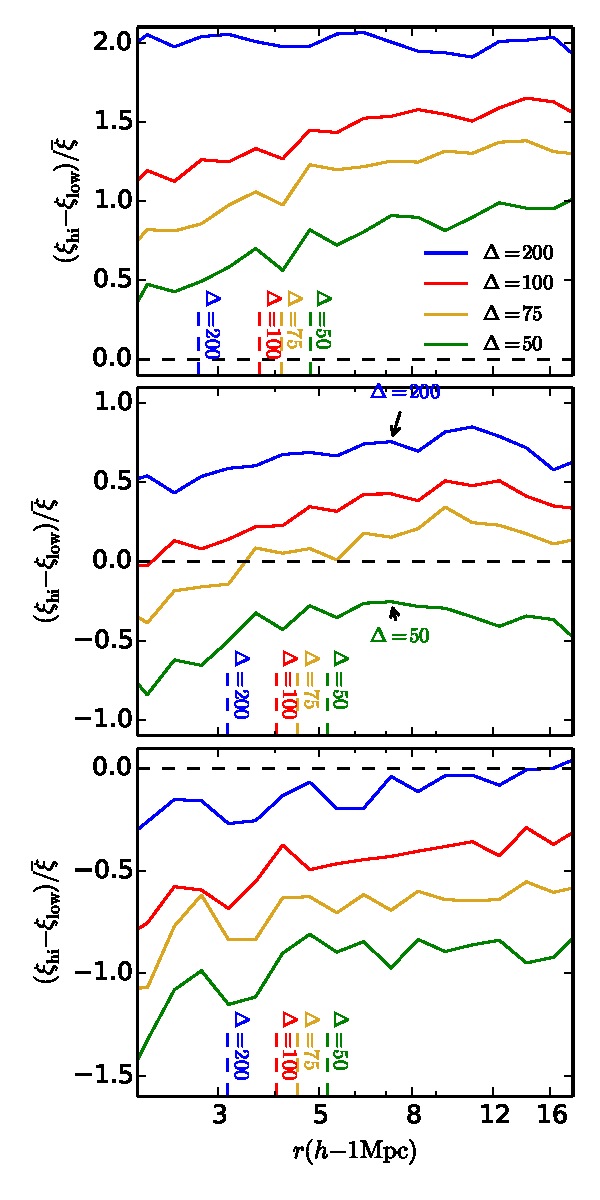
\includegraphics[width=.4\textwidth]{all_cfhilow_z00_cutcomp.pdf}
	\caption{The difference of the correlation function for only the top 20\% most concentrated halos and the bottom 20\% in concentration, normalized by the overall correlation function of the entire sample. From top to bottom we show the results for the lowest mass cut in \simA, \simB, and \simC \ that excludes ill resolved halos. The dashed lines along the bottom denote the largest halo radius for a given value of the overdensity parameter.}
	\label{fig:cc_cfcompare}
\end{figure}

%% note: we need to remake this plot!

The left column of Figure~\ref{fig:cc_cfcompare} demonstrates the results of our method as we change the value of $\Delta$. We see that when we are interested in studying primarily a sample of low mass halos, such as in in \simA, it is difficult to use this method to account for assembly bias for any reasonable matter. However, when looking at a more reasonable mass range, there is a removal of assembly bias on large scales between $\Delta = 75$ and $\Delta=50$ that can be noted in the data. It should be noted that this is effectively a ``sweet spot'' effect, where decreasing the value of $\Delta$ (or correspondingly, the size of an average halo) will start to give increasing amounts of power in the correlation function to the least concentrated halos - essentially introducing a new assembly bias. The physical nature of this is of interest to us, and we attempt to present an intuitive sense of the effect further on. Furthermore, we note that when interest is focused on the most massive halos, assembly bias appears to be minimal in terms of the clustering for the largest scales with the standard definition, perhaps giving a more statistical motivation to the use of $\Delta = 200$.

\begin{figure}
	\centering
	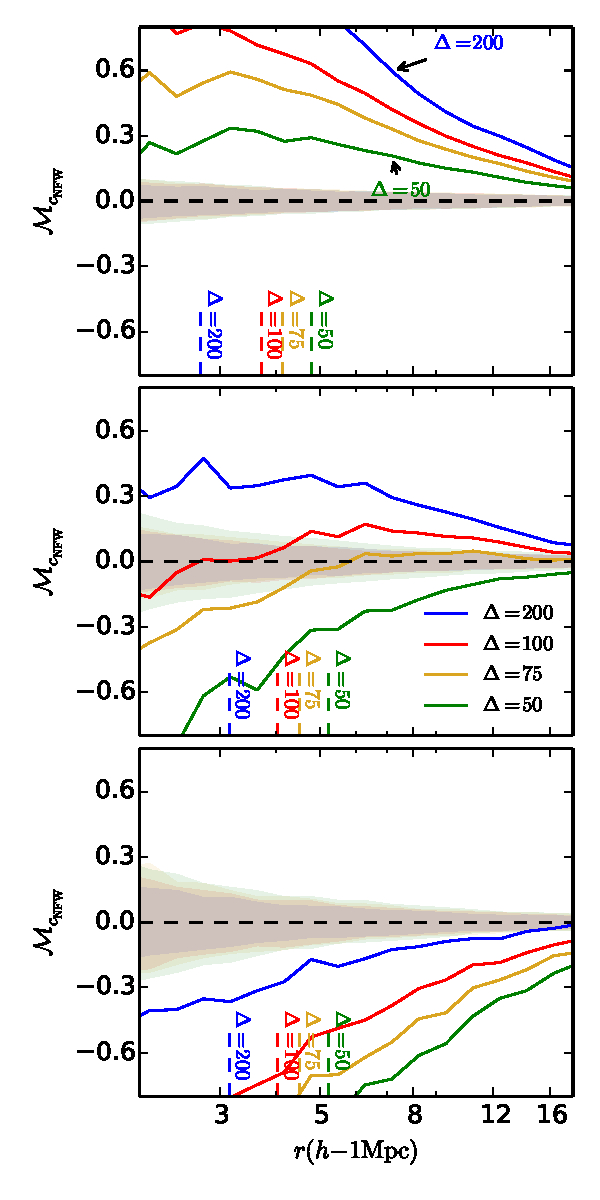
\includegraphics[width=.4\textwidth]{all_mcf_cnfw_z00_cutcomp.pdf}
	\caption{The marked correlation function for the concentration defined according to the NFW profile. From top to bottom we show the results for the lowest mass cut in \simA, \simB, and \simC \ that excludes ill resolved halos. The shaded bands represent 2-sigma confidence regions generated by randomization of the marks. The dashed lines along the bottom denote the largest halo radius for a given value of the overdensity parameter.}
	\label{fig:cc_mcf_cnfw}
\end{figure}

The NFW defined concentration MCF is shown in the left column of Figure~\ref{fig:cc_mcf_cnfw}. It can been that as we decrease the value of the overdensity parameter $\Delta$ to lower values down to $\Delta = 50$, the assembly bias trend can be reduced and even reduced. It can be seen that at scales of $r > 10 \hMpc$, environmental effects are removed between $\Delta = 75$ and $\Delta = 50$ for \simB, as noted before. This is repeated for the velocity ratio defined concentration in the left column of Figure~\ref{fig:cc_mcf_cV}. It again demonstrates that the same values of $\Delta$ are preferred for the removal of assembly bias as with the NFW concentration. This seems to indicate that our methodology should be effective at minimizing the impact of assembly bias at large scales.

\begin{figure}
	\centering
	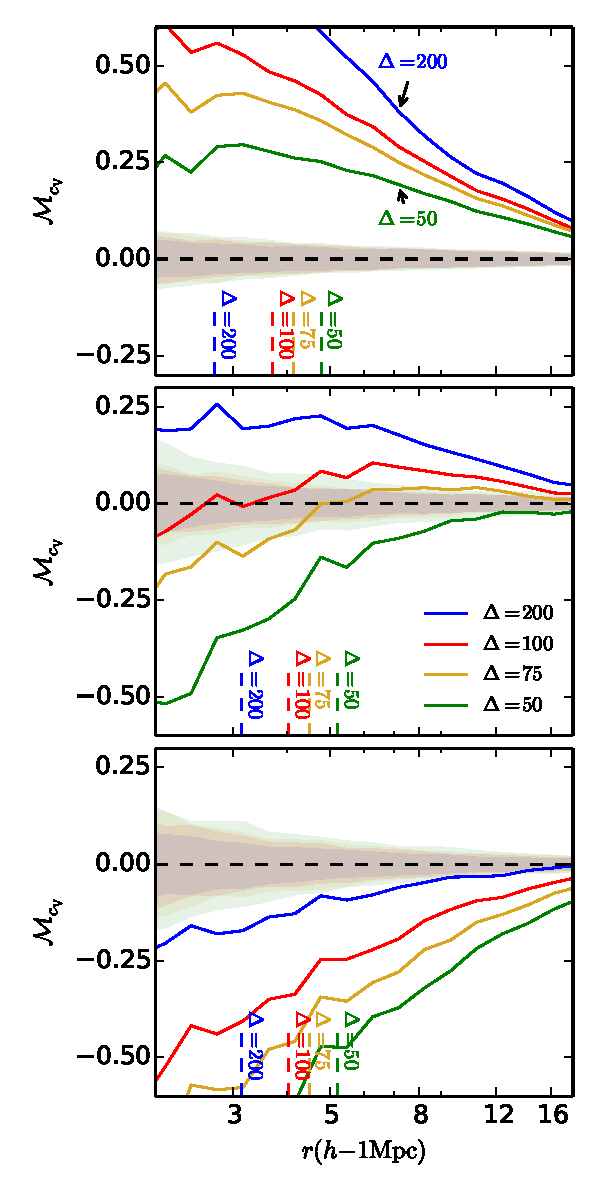
\includegraphics[width=.4\textwidth]{all_mcf_cV_z00_cutcomp.pdf}
	\caption{The marked correlation function for the concentration defined according to the velocity ratio. From top to bottom we show the results for the lowest mass cut in \simA, \simB, and \simC \ that excludes ill resolved halos. The shaded bands represent 2-sigma confidence regions generated by randomization of the marks. The dashed lines along the bottom denote the largest halo radius for a given value of the overdensity parameter.}
	\label{fig:cc_mcf_cV}
\end{figure}

\begin{figure}
	\centering
	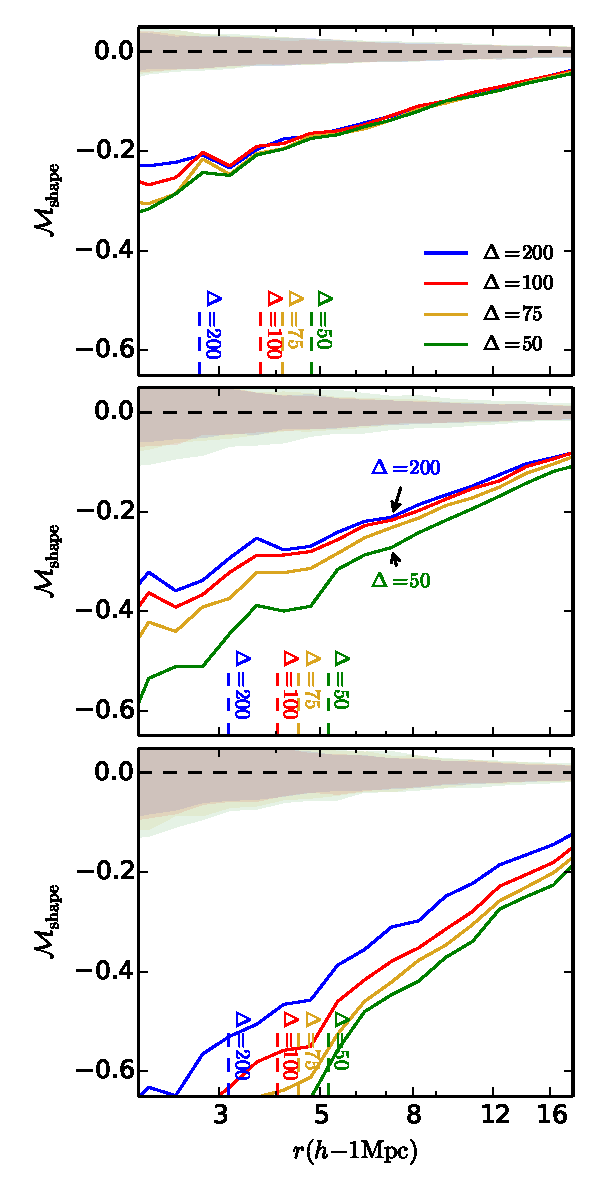
\includegraphics[width=.4\textwidth]{all_mcf_s_z00_cutcomp.pdf}
	\caption{The marked correlation function for the shape of the halo. From top to bottom we show the results for the lowest mass cut in \simA, \simB, and \simC \ that excludes ill resolved halos. The shaded bands represent 2-sigma confidence regions generated by randomization of the marks. The dashed lines along the bottom denote the largest halo radius for a given value of the overdensity parameter.}
	\label{fig:cc_mcf_s}
\end{figure}

The left column of Figure~\ref{fig:cc_mcf_s} demonstrates a case in which the halo property does not have environmental dependence removed under our simple method of halo redefinition. In particular, with decreasing values of $\Delta$, we only serve to increase the strength of this environmental dependence. This result seems to indicate a process occurring to drive the shape of the halo is on scales that are significantly larger than the size of the halo, such that our method will not be able to encompass these effects. A similar result is located in both the left columns of Figure~\ref{fig:cc_mcf_spin} and Figure~\ref{fig:cc_mcf_nsat}, in which the spin parameter mark and satellite number mark experience the exact same effect.

\begin{figure}
	\centering
	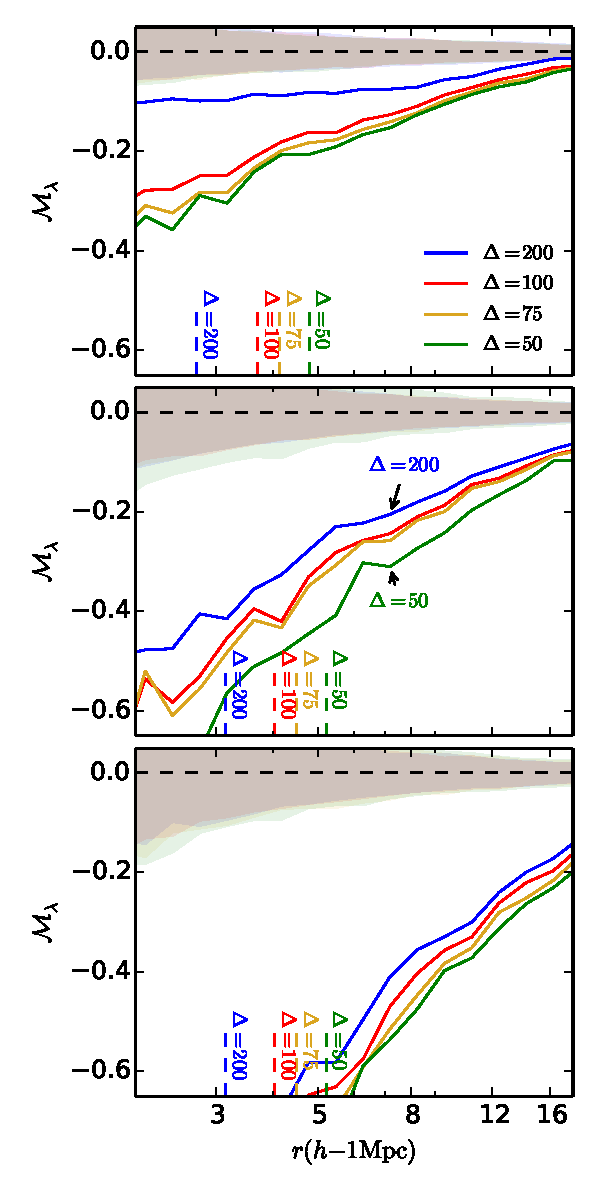
\includegraphics[width=.4\textwidth]{all_mcf_spin_z00_cutcomp.pdf}
	\caption{The marked correlation function for the spin parameter of the halo. From top to bottom we show the results for the lowest mass cut in \simA, \simB, and \simC \ that excludes ill resolved halos. The shaded bands represent 2-sigma confidence regions generated by randomization of the marks. The dashed lines along the bottom denote the largest halo radius for a given value of the overdensity parameter.}
	\label{fig:cc_mcf_spin}
\end{figure}

\begin{figure}
	\centering
	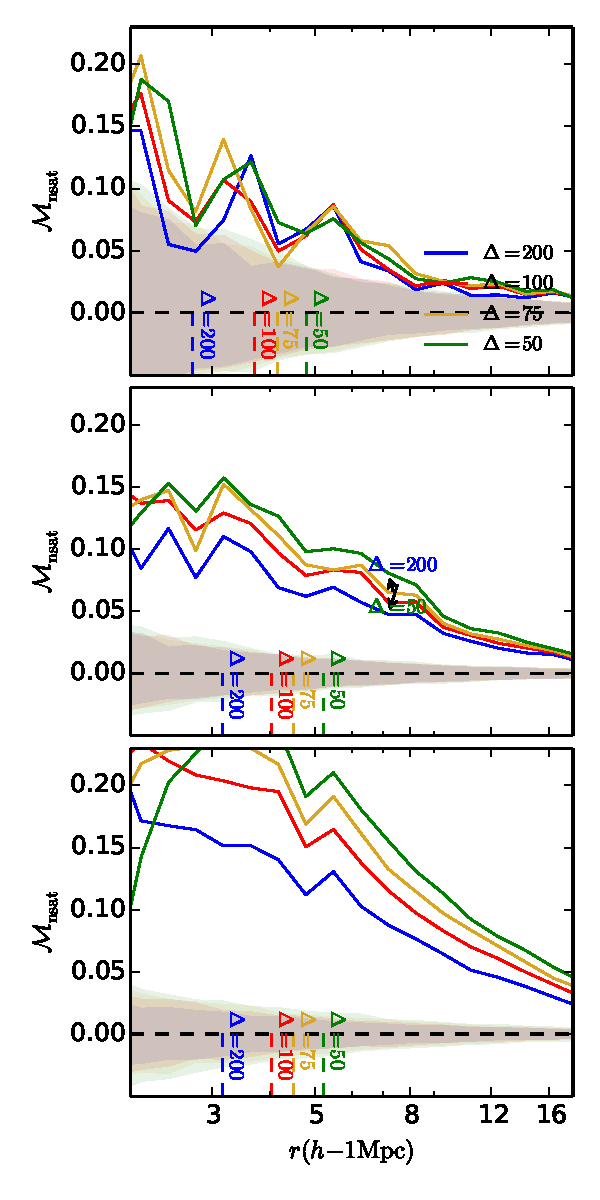
\includegraphics[width=.4\textwidth]{all_mcf_nsat_z00_cutcomp.pdf}
	\caption{The marked correlation function for the number of satellites for a host halo. From top to bottom we show the results for the lowest mass cut in \simA, \simB, and \simC \ that excludes ill resolved halos. The shaded bands represent 2-sigma confidence regions generated by randomization of the marks. The dashed lines along the bottom denote the largest halo radius for a given value of the overdensity parameter.}
	\label{fig:cc_mcf_nsat}
\end{figure}

Overall, while some statistics of the halo can be made to become independent of environmental effects, there exist several that cannot. These environmental effects are not negligible when considering applications of the halo model. In contrast, if one is only interested in the concentration of the halo, it is feasible to take advantage of our methodology in order to remove environmental effects. In contrast, it is not possible to apply the halo model directly to statistics such as the number of satellite halos or the shape without accounting for these environmental effects. We do not yet have a full understanding of what leads to the visible effects that we see on some of these marks, but we present a series of cases in which an intuitive understanding may be gained as to the root causes.

We would also like to study our sample for some insight as to how this process of correction is actually functioning. For example, we would like to know if it is a more careful selection of halos in our simulation that results in the removal of this apparent assembly bias or if it is the increased noise in the statistics as a result of reducing the number of halos. There is also the possibility of halo statistics changing as a result of the new halo definitions to be considered. One can imagine that the addition of a large amount of mass toward the edge of the halo would reasonably change measures of concentration, shape, and spin. To test some of these possibilities, we run an algorithm to match halos across our multiple catalogs. We identify halos that are within a distance tolerance that we scale such that there are no identifications of multiple halos to the same object in another catalog. Catalogs are all matched against a single target catalog. This target catalog is chosen to fit the value of $\Delta$ that we find best removes assembly bias in large scales for the concentration marks chosen. For the \citet{diemer15} simulations, we find this to be a value of approximately $\Delta = 70$. Once the catalogs have been matched against this primary catalog, we rerun our marked correlation function calculations using only host halos identified across both catalogs. This tests if the exclusion of halos that are subsumed in the lower $\Delta$ catalog is the primary cause of our results as well as those halos that are commonly referred to as backsplash halos.

We can see the results of this test in Figure~\ref{fig:hvm_cfcompare} through Figure~\ref{fig:hvm_mcf_nsat}. Comparing in each case, the $\Delta = 200$ result when utilizing a catalog matched to our best fit $\Delta$ demonstrates less assembly bias than the full catalog for the mass cut would demonstrate for our concentration marks. While the magnitude of this result does vary with scale, upwards of 80\% of assembly bias can be accounted for as a result of this selection effect. Furthermore, most of the removed assembly bias occurs on scales that are comparable to the increase in the halo radius between the samples. This seems to indicate that there is significant contamination of host halo statistics by backsplash halos and other halos that would be subsumed into a common host given an increase in halo size.

\begin{figure*}
	\centering
	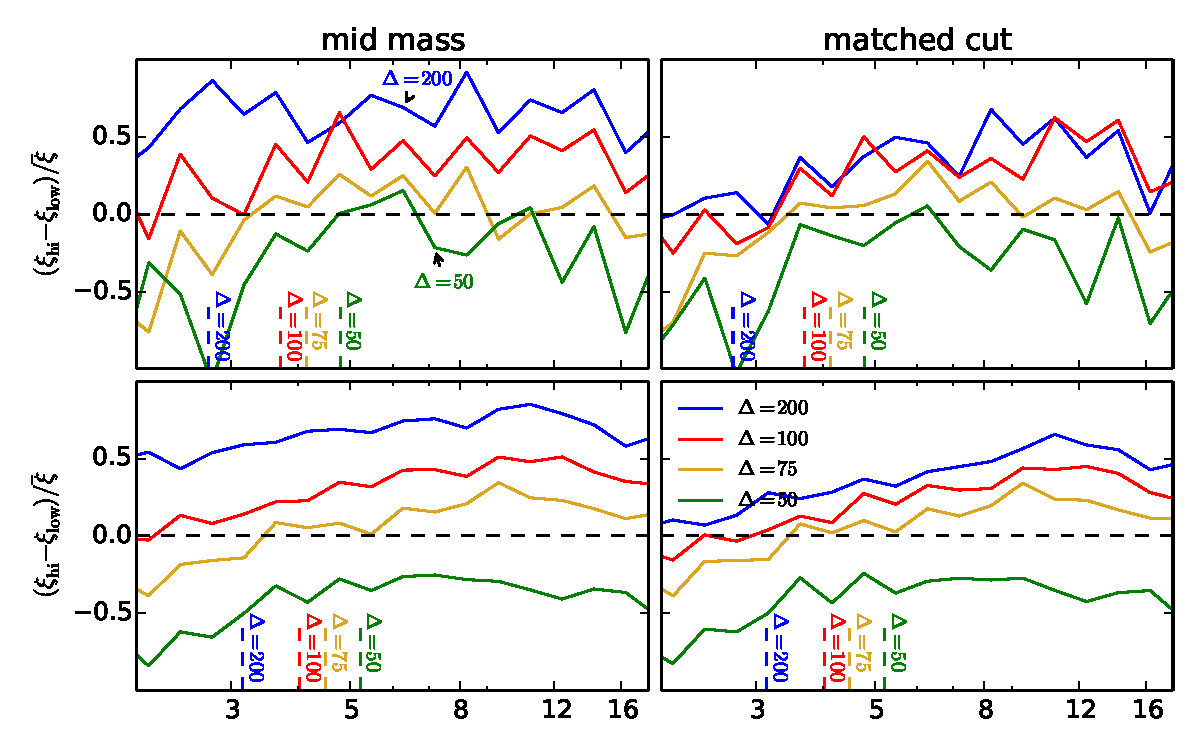
\includegraphics[width=.9\textwidth]{all_cfhilow_z00_hostsvmatch.pdf}
	\caption{The difference of the correlation function for only the top 20\% most concentrated halos and the bottom 20\% in concentration, normalized by the overall correlation function of the entire sample. The left (right) panel shows the ``mid mass'' (``matched'') cut on \simA \ and \simB. The ``matched'' cut accounts for potential backsplash halos, as discussed further in the text. The dashed lines along the bottom denote the largest halo radius for a given value of the overdensity parameter.}
	\label{fig:hvm_cfcompare}
\end{figure*}

\begin{figure*}
	\centering
	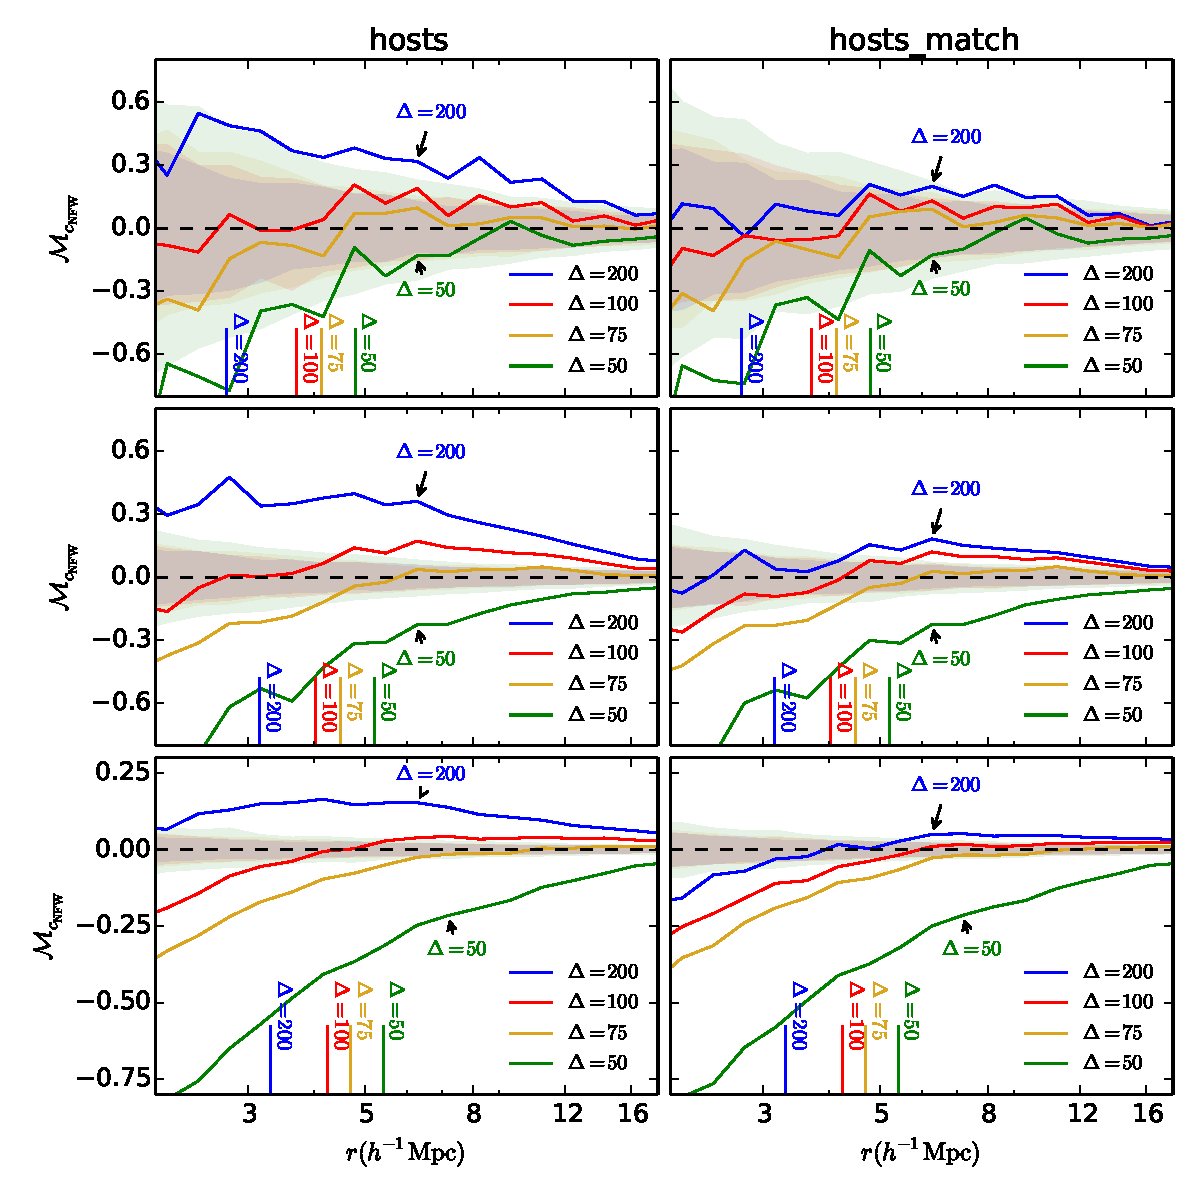
\includegraphics[width=.9\textwidth]{all_mcf_cnfw_z00_hostsvmatch.pdf}
	\caption{The marked correlation function for the concentration defined according to the NFW profile. The left (right) panel shows the ``mid mass'' (``matched'') cut on \simA \ and \simB. The ``matched'' cut accounts for potential backsplash halos, as discussed further in the text. The dashed lines along the bottom denote the largest halo radius for a given value of the overdensity parameter.}
	\label{fig:hvm_mcf_cnfw}
\end{figure*}

\begin{figure*}
	\centering
	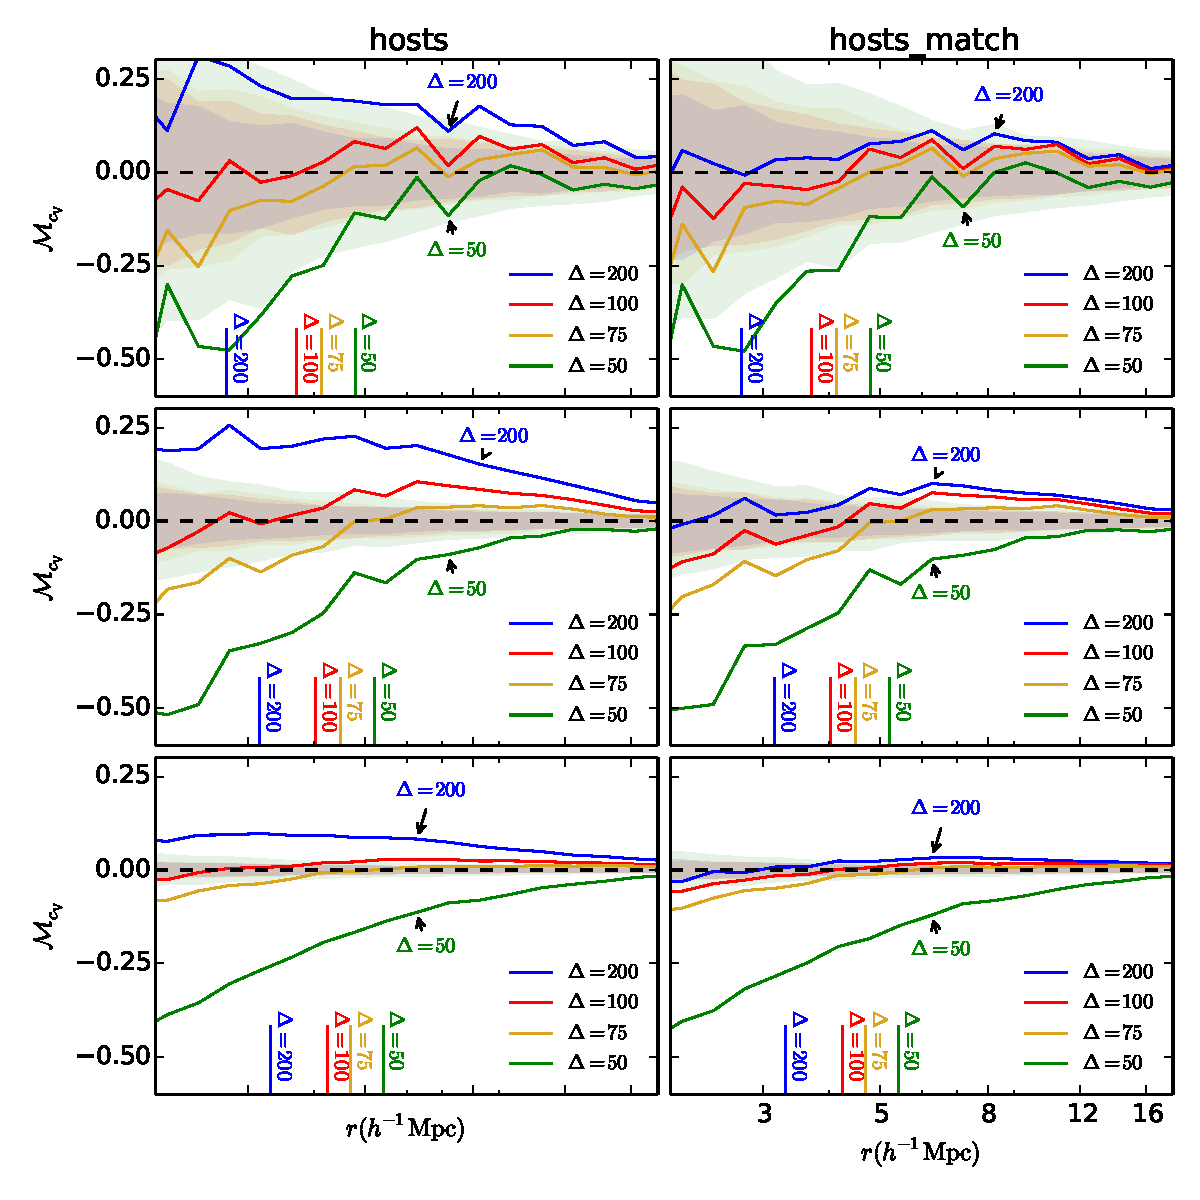
\includegraphics[width=.9\textwidth]{all_mcf_cV_z00_hostsvmatch.pdf}
	\caption{The marked correlation function for the concentration defined according to the velocity ratio. The left (right) panel shows the ``mid mass'' (``matched'') cut on \simA \ and \simB. The ``matched'' cut accounts for potential backsplash halos, as discussed further in the text. The dashed lines along the bottom denote the largest halo radius for a given value of the overdensity parameter.}
	\label{fig:hvm_mcf_cV}
\end{figure*}

\begin{figure*}
	\centering
	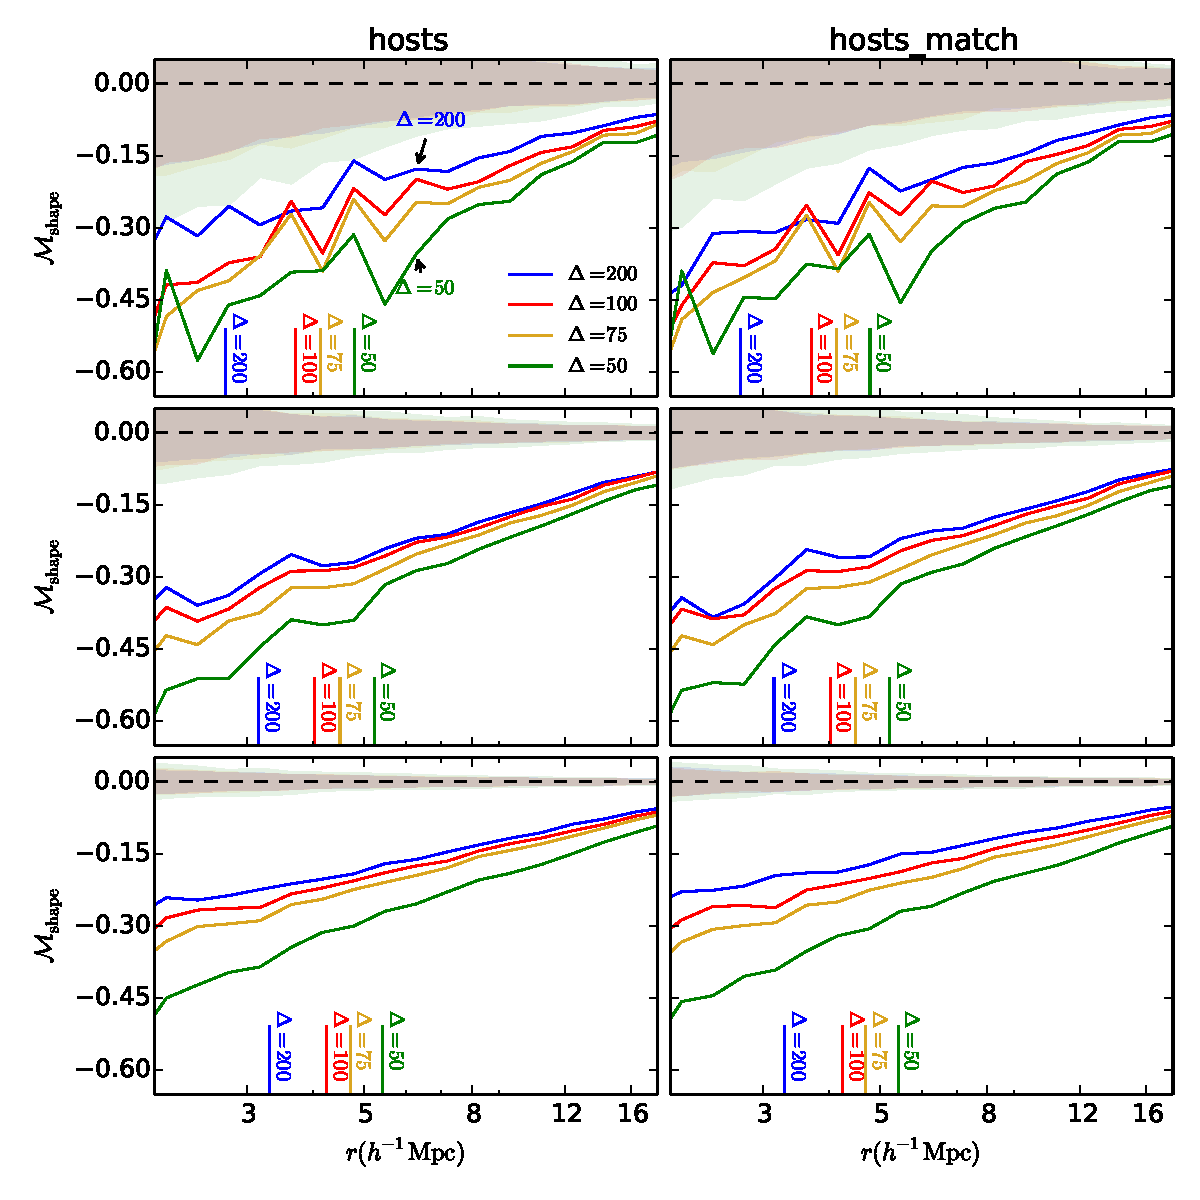
\includegraphics[width=.9\textwidth]{all_mcf_s_z00_hostsvmatch.pdf}
	\caption{The marked correlation function for the shape parameter. The left (right) panel shows the ``mid mass'' (``matched'') cut on \simA \ and \simB. The ``matched'' cut accounts for potential backsplash halos, as discussed further in the text. The dashed lines along the bottom denote the largest halo radius for a given value of the overdensity parameter.}
	\label{fig:hvm_mcf_s}
\end{figure*}

\begin{figure*}
	\centering
	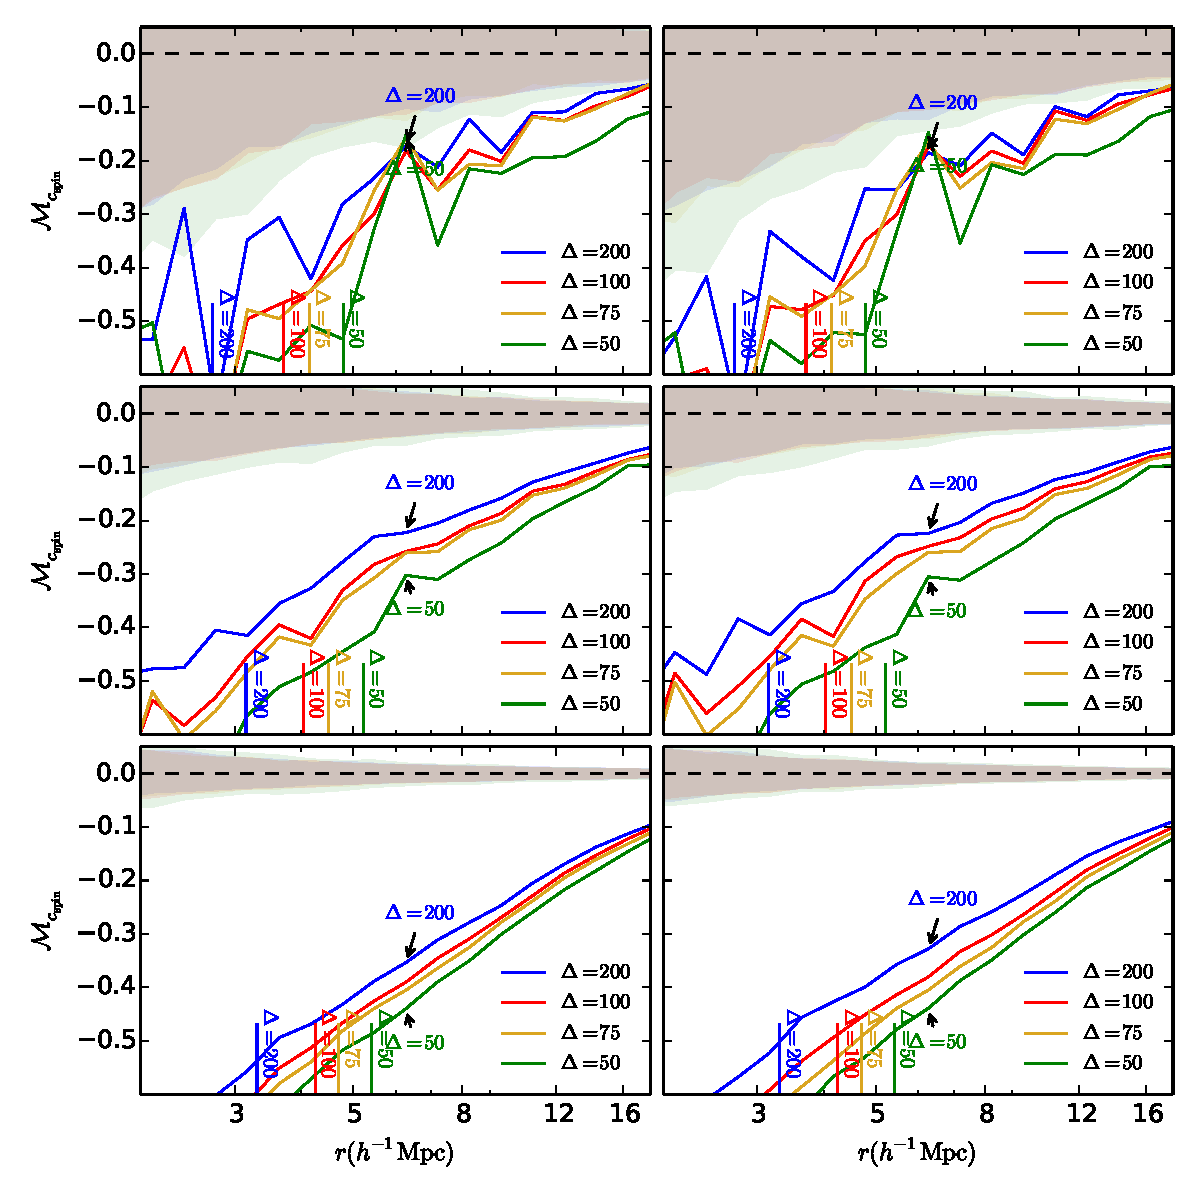
\includegraphics[width=.9\textwidth]{all_mcf_spin_z00_hostsvmatch.pdf}
	\caption{The marked correlation function for the spin parameter. The left (right) panel shows the ``mid mass'' (``matched'') cut on \simA \ and \simB. The ``matched'' cut accounts for potential backsplash halos, as discussed further in the text. The dashed lines along the bottom denote the largest halo radius for a given value of the overdensity parameter.}
	\label{fig:hvm_mcf_spin}
\end{figure*}

\begin{figure*}
	\centering
	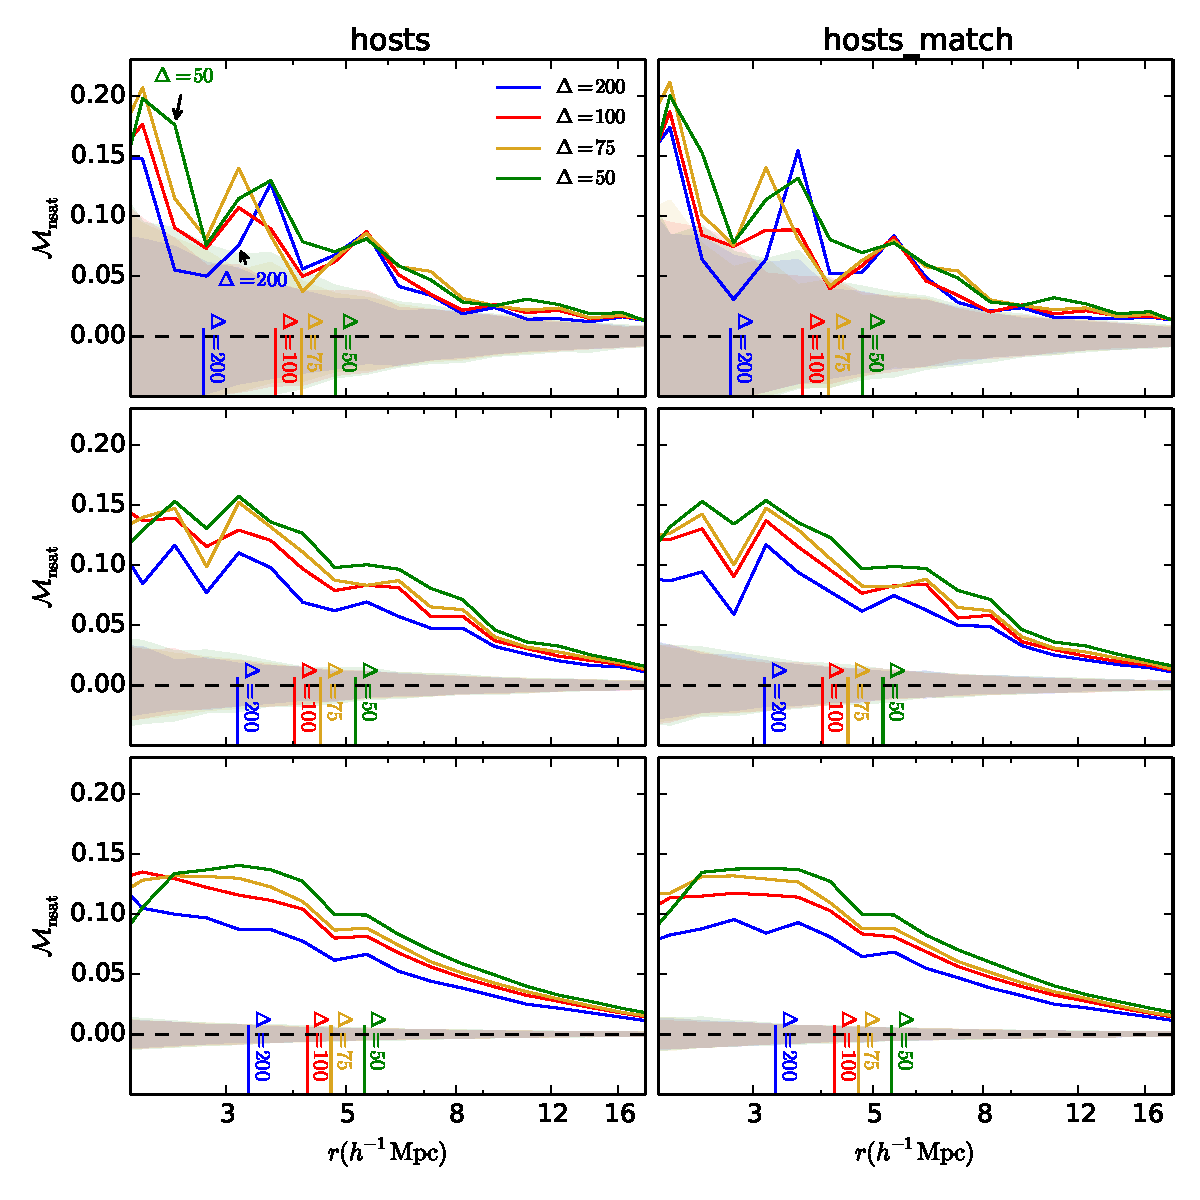
\includegraphics[width=.9\textwidth]{all_mcf_nsat_z00_hostsvmatch.pdf}
	\caption{The marked correlation function for the satellite number. The left (right) panel shows the ``mid mass'' (``matched'') cut on \simA \ and \simB. The ``matched'' cut accounts for potential backsplash halos, as discussed further in the text. The dashed lines along the bottom denote the largest halo radius for a given value of the overdensity parameter.}
	\label{fig:hvm_mcf_nsat}
\end{figure*}

However, it is worth noting that statistics such as spin parameter, shape, and satellite numbers do not benefit from this selection effect. Assembly bias in these statistics remains nearly identical, suggesting that the selection effects that preferentially account for backsplash halos do not impact these marks. This does serve as a consistency check: given that our methodology does not seem to have a positive impact on the behavior of these marks, the fact that this selection criteria would have positive impact on the data would be an oddity. Instead, we have another confirmation as to the intrinsic ties between these halo statistics and environment.

Given that the removal of assembly bias is not being driven by introducing noice, we now will attempt to determine why the different marks exhibit different behaviors. The first interesting feature is how well our two separate definitions of concentration interact with each other. In the case that the halo can be described well by an NFW profile, one expects a direct relationship between the NFW defined halo concentration and the velocity ratio defined halo concentration. While some variation can be expected due to halos not perfectly being fit by an NFW profile, we do see that the features in one concentration proxy are mirrored in the other. This allows for the two concentration markers to support each other well with regards to our ability to remove environmental effects on large scales.

Halo shape and satellite number are statistics that do not end up having their environmental effects removed and can even be made more prominent by our methodology. One intuitive way to consider the former statistic is in the context of the cosmic web. Studies have shown a statistically significant alignment between filaments and satellite galaxy position \citep{tempel15, velliscig15}. Our method then expands the halo radius and subsumes material that was previously outside of the halo. A simple graphic illustrates this potential effect in Figure~\ref{fig:plotcircles}. As there is a preferential distribution of these satellites that are being subsumed into the halo, this would serve to induce a shape to the halo that would then be determined by Rockstar. In addition, as our satellite number is chosen by those halos within the halo radius, we anticipate that the most clustered regions would see the largest increase in satellite count and thus see an increase in the satellite number mark.

The ``sweet spot'' behavior of this method is also of interest to us. The halo redefinition process that we use serves to decrease halo clustering for the most concentrated halos and increase halo clustering for the least concentrated halos. In the case of the high concentration cut, the reduced clustering can be seen as a result of halo exclusion. As we exchange collections of tightly clustered smaller halos for a single larger halo, then the most prominent contribution of the two-point correlation function will be reduced at all scales. Furthermore, it suggests that the assembly bias that we witness is correlated with the choice of halo definition. This effect may be necessary to explaining the mixed results in the field at determining just how strong assembly bias is.

\begin{figure*}
	\centering
	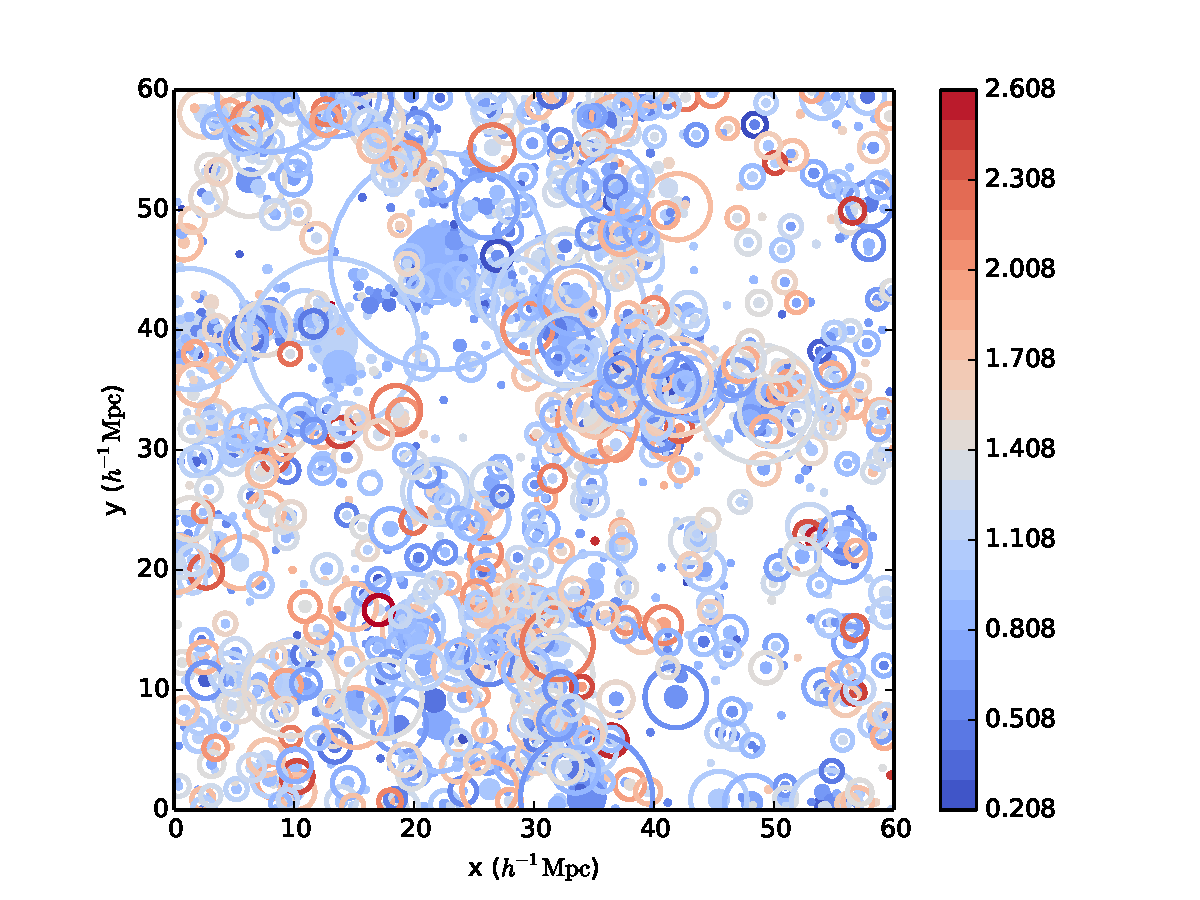
\includegraphics[width=.9\textwidth]{plotcircles_coolwarm.pdf}
	\caption{A $20 \hMpc$ deep cut of \simB \ along the z-axis. This zoom-in demonstrates the process that decreases the shape parameter as a function of clustering. The size of each circle represents the projection of a spherical dark matter halo with a given halo radius onto the x-y plane. Filled circles use the $\Delta = 200$ catalog and unfilled circles use the $\Delta = 10$ catalog in order to make the effect more visible. Color scale refers to the log shape mark, normalized by halos of the same mass.}
	\label{fig:plotcircles}
\end{figure*}

%% another thing to repeat on one of the Diemer boxes. High priority.

Given the differences between the simulation results and with the data available to us with the \citet{diemer15} simulations, we then explore the effect of the choice in mass cut. The low mass cut effects are shown in the Figure~\ref{fig:hvl_cfcompare} through Figure~\ref{fig:hvl_mcf_nsat}. This cut explores the area in which we are including ill-resolved halos potentially into the simulation. Namely, utilizing this mass cut on \simB \ data includes halos that do not fit the form of the expected monotonic halo mass-concentration relation. We can determine several facts from this exercise in resolution testing. The first is that the general behavior of the marks seems to be the same regardless of the influence of the resolution effects. Decreasing the value of $\Delta$ still moves our marked correlation functions in the same directions as the previous mass cut, although often from a very different starting location. Even with potentially ill resolved objects, the method can be brought to bear upon the problem - potentially a concern if the simulation's ability to resolve a particular statistic is questionable. Also noteable is that the level of the assembly bias is reduced in the case of this lower mass cut in \simB \ when compared to \simA. This is distinctly different from our previous example, in which both \simA \ and \simB \ both contain only well resolved halos within the mass cut and have nearly identical assembly bias at every scale, aside from simulation noise. This seems to imply that including unphysical halos in our sample makes it difficult to determine the actual assembly bias at work.

\begin{figure*}
	\centering
	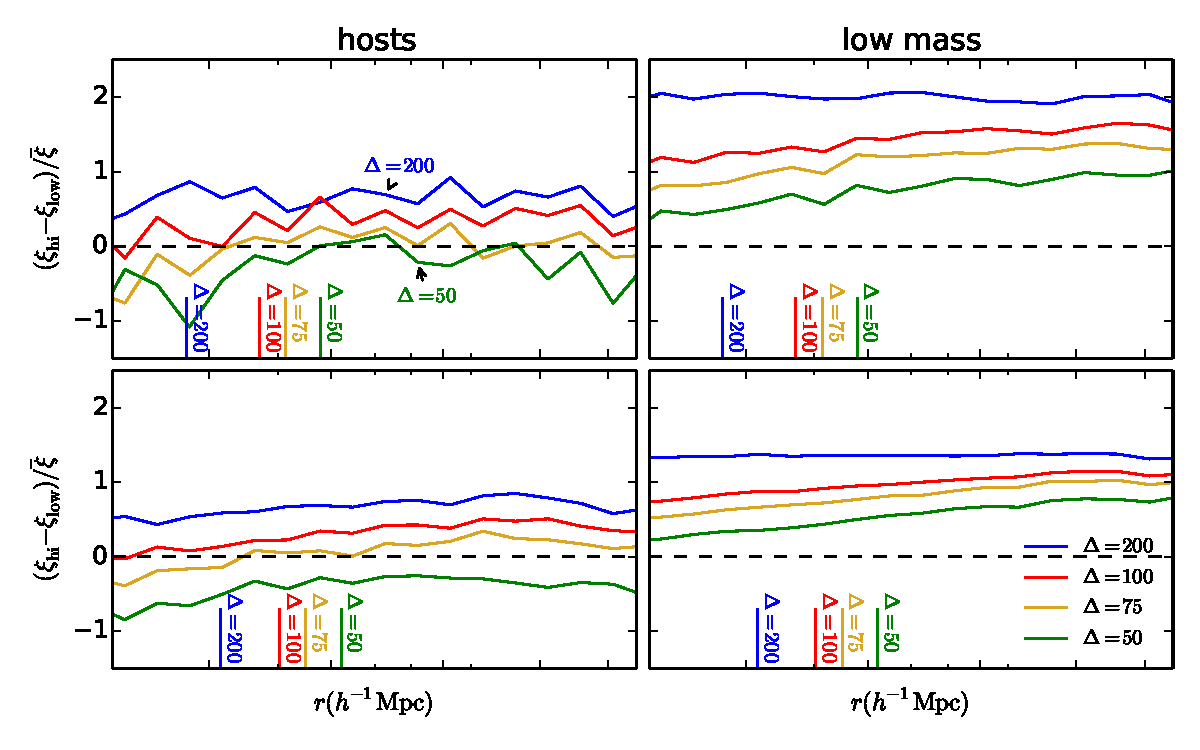
\includegraphics[width=.9\textwidth]{all_cfhilow_z00_hostsvlow.pdf}
	\caption{The difference of the correlation function for only the top 20\% most concentrated halos and the bottom 20\% in concentration, normalized by the overall correlation function of the entire sample. The top row uses \simA \  data while the bottom row uses \simB \ data. The left column utilizes the ``mid mass'' cutoff, while the right column demonstrates the ``low mass'' cutoff. The dashed lines along the bottom denote the largest halo radius for a given value of the overdensity parameter}
	\label{fig:hvl_cfcompare}
\end{figure*}

\begin{figure*}
	\centering
	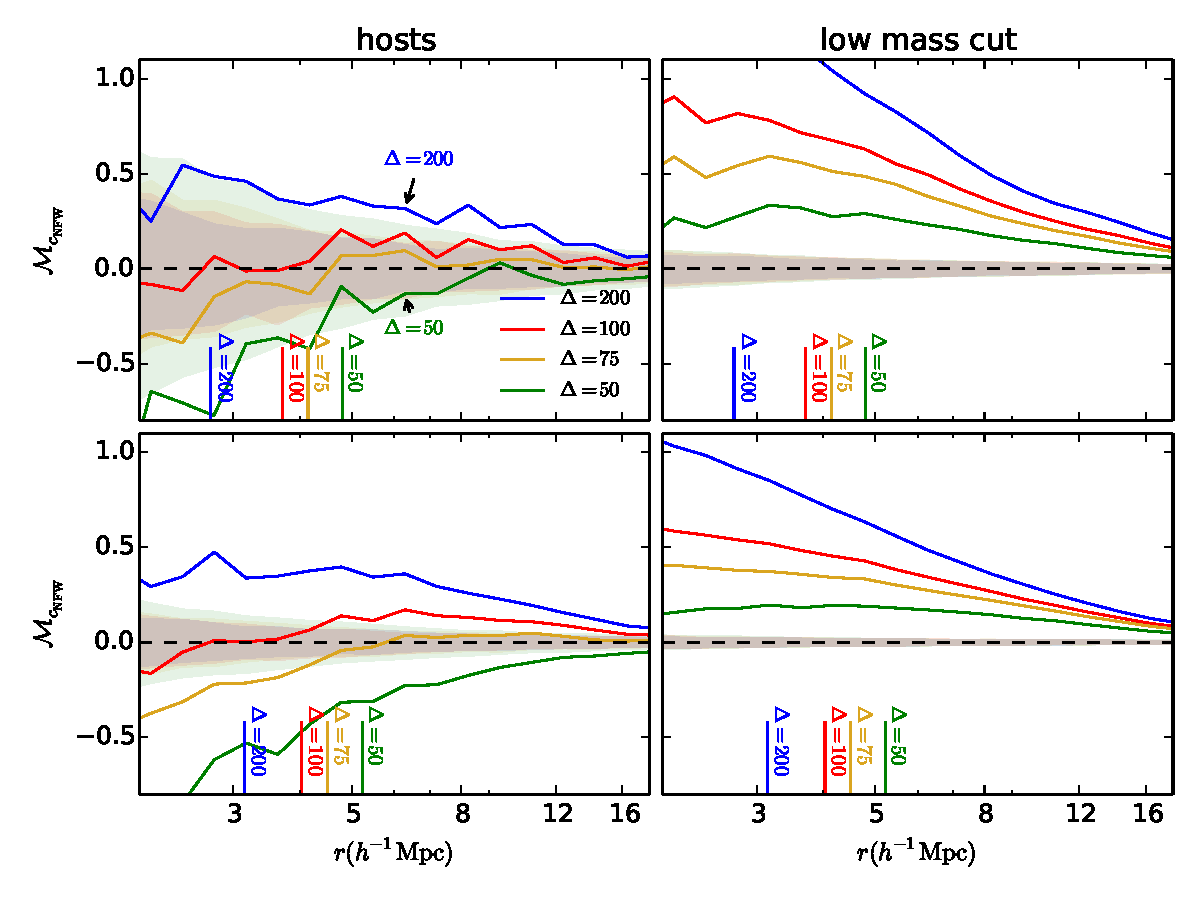
\includegraphics[width=.9\textwidth]{all_mcf_cnfw_z00_hostsvlow.pdf}
	\caption{Comparison of the marked correlation function for the concentration defined according to the NFW profile between the ``mid mass'' cutoff (left column) and the ``low mass'' cutoff (right column). The top row uses \simA \ data while the bottom row uses \simB \ data. The shaded bands represent 2-sigma confidence regions generated by randomization of the marks. The dashed lines along the bottom denote the largest halo radius for a given value of the overdensity parameter.}
	\label{fig:hvl_mcf_cnfw}
\end{figure*}

\begin{figure*}
	\centering
	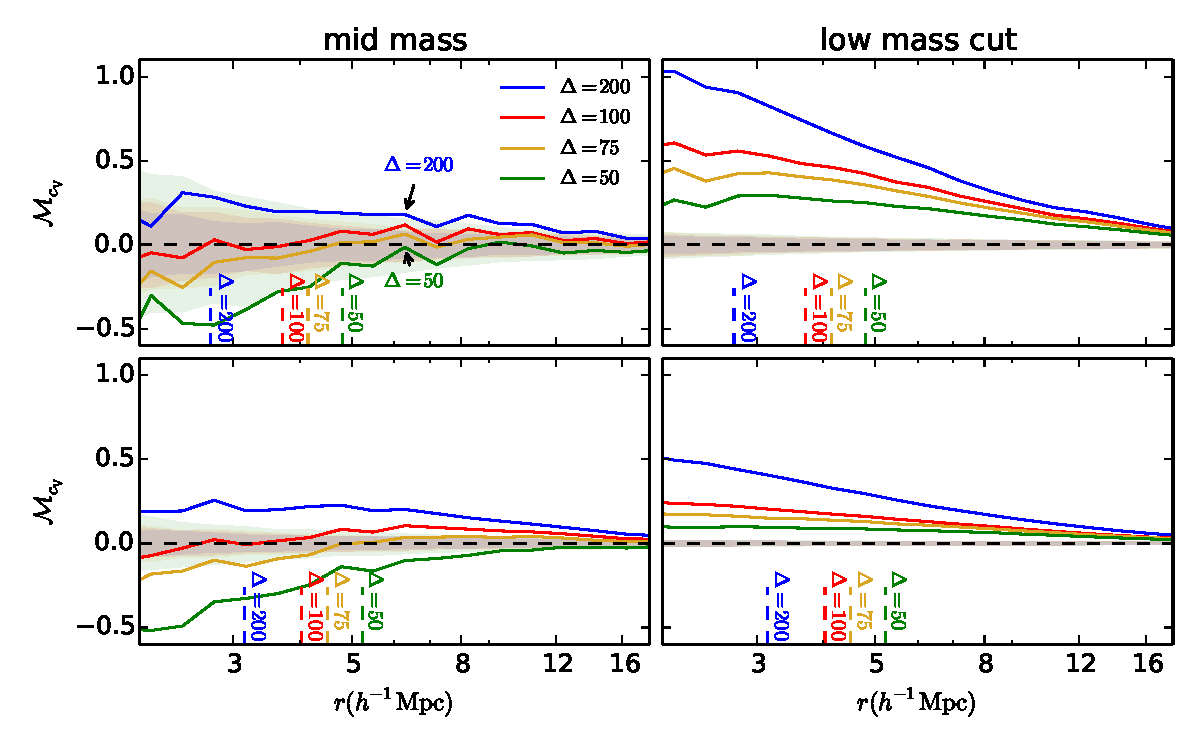
\includegraphics[width=.9\textwidth]{all_mcf_cV_z00_hostsvlow.pdf}
	\caption{Comparison of the marked correlation function for the concentration defined according to the velocity ratio between the ``mid mass'' cutoff (left column) and the ``low mass'' cutoff (right column). The top row uses \simA \ data while the bottom row uses \simB \ data. The shaded bands represent 2-sigma confidence regions generated by randomization of the marks. The dashed lines along the bottom denote the largest halo radius for a given value of the overdensity parameter.}
	\label{fig:hvl_mcf_cV}
\end{figure*}

\begin{figure*}
	\centering
	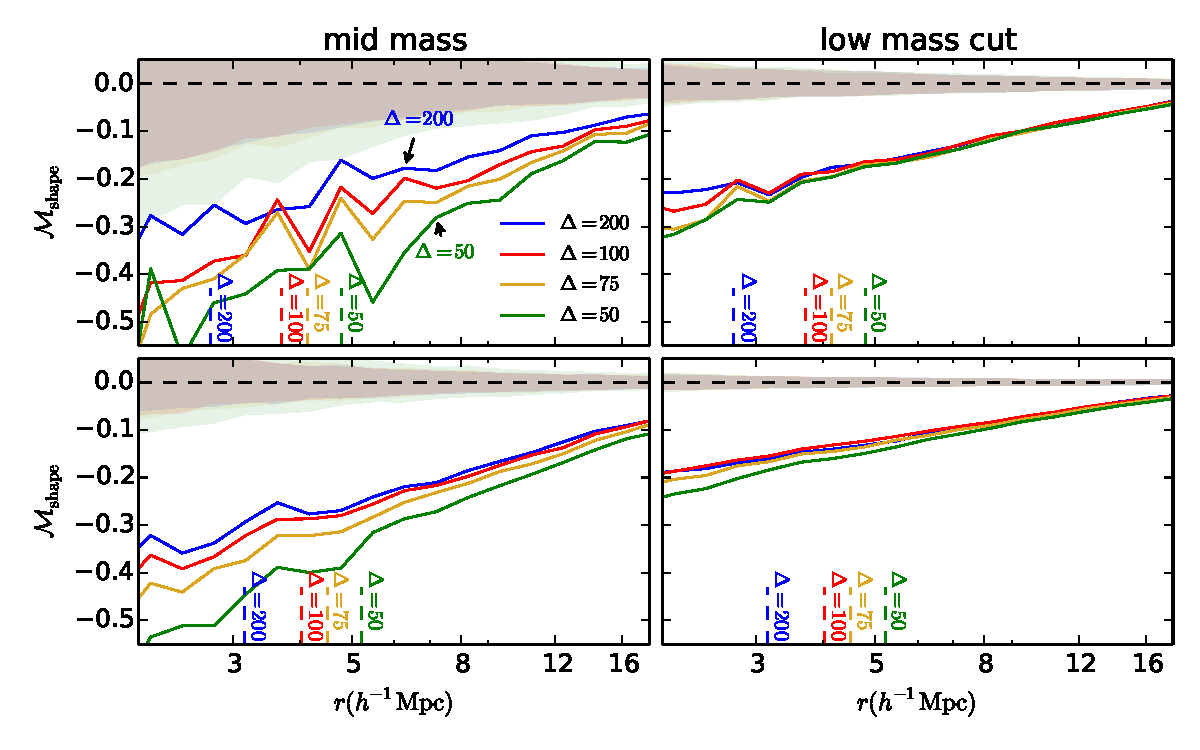
\includegraphics[width=.9\textwidth]{all_mcf_s_z00_hostsvlow.pdf}
	\caption{Comparison of the marked correlation function for the shape of the halo between the ``mid mass'' cutoff (left column) and the ``low mass'' cutoff (right column). The top row uses \simA \ data while the bottom row uses \simB \ data. The shaded bands represent 2-sigma confidence regions generated by randomization of the marks. The dashed lines along the bottom denote the largest halo radius for a given value of the overdensity parameter.}
	\label{fig:hvl_mcf_s}
\end{figure*}

\begin{figure*}
	\centering
	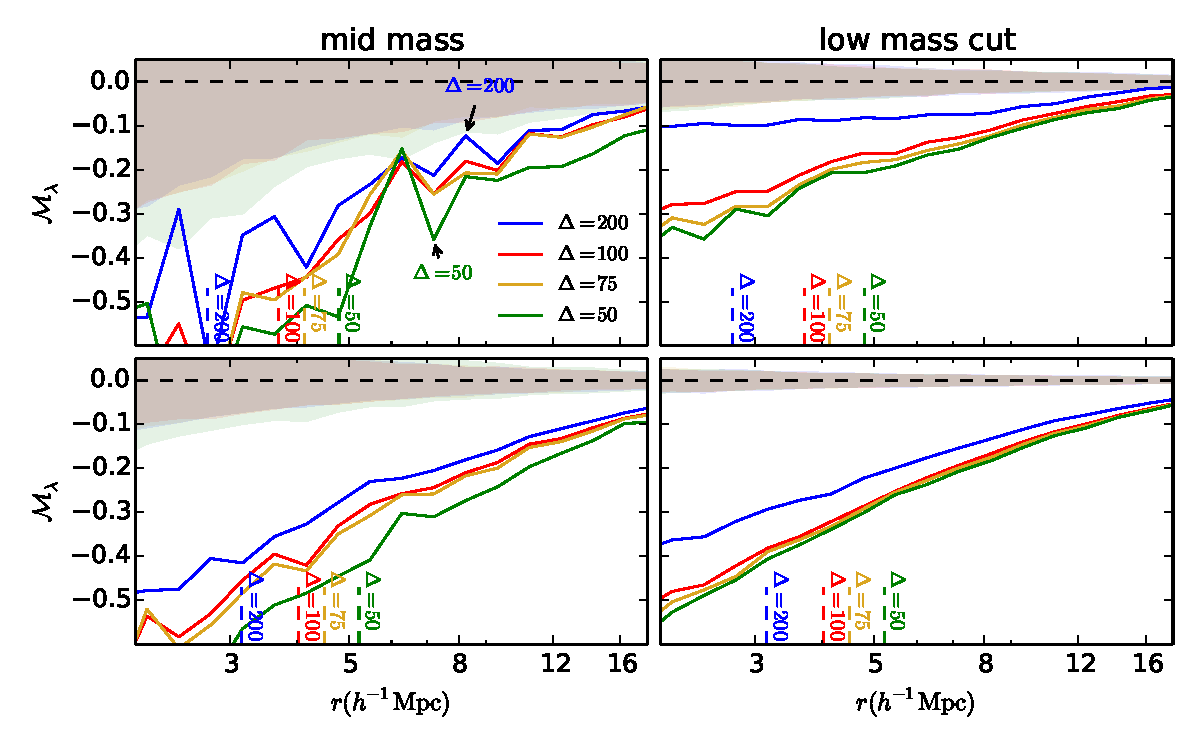
\includegraphics[width=.9\textwidth]{all_mcf_spin_z00_hostsvlow.pdf}
	\caption{Comparison of the marked correlation function for the spin of the halo between the ``mid mass'' cutoff (left column) and the ``low mass'' cutoff (right column). The top row uses \simA \ data while the bottom row uses \simB \ data. The shaded bands represent 2-sigma confidence regions generated by randomization of the marks. The dashed lines along the bottom denote the largest halo radius for a given value of the overdensity parameter.}
	\label{fig:hvl_mcf_spin}
\end{figure*}

\begin{figure*}
	\centering
	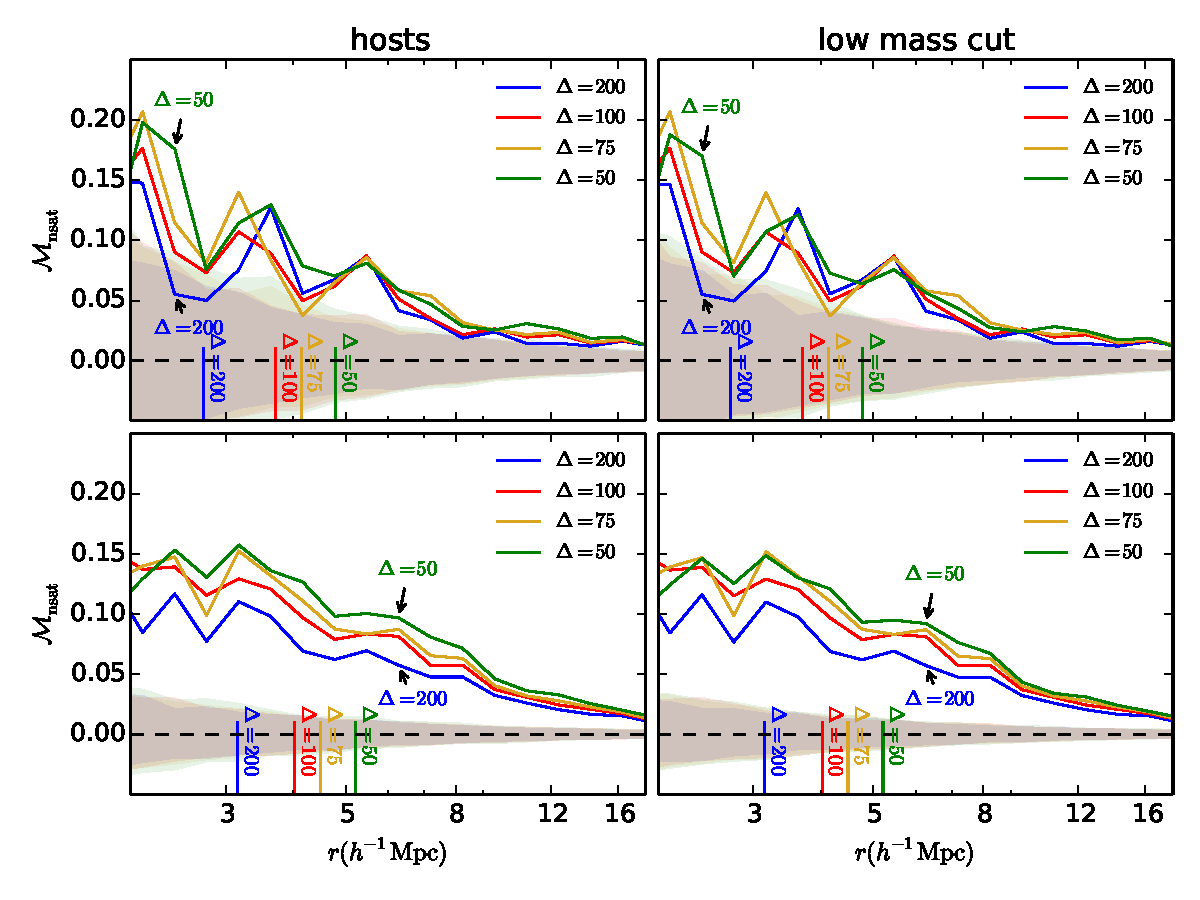
\includegraphics[width=.9\textwidth]{all_mcf_nsat_z00_hostsvlow.pdf}
	\caption{Comparison of the marked correlation function for the satellite number between the ``mid mass'' cutoff (left column) and the ``low mass'' cutoff (right column). The top row uses \simA data while the bottom row uses \simB data. The shaded bands represent 2-sigma confidence regions generated by randomization of the marks. The dashed lines along the bottom denote the largest halo radius for a given value of the overdensity parameter.}
	\label{fig:hvl_mcf_nsat}
\end{figure*}

We can repeat this exercise by looking at a different set of mass cuts. In this case we will utilize our highest mass cut on \simB and \simC. This case does not include poorly resolved halos as we were including in the previous example. Instead, the smaller sized box runs the risk of having less of the most massive halos, resulting in having a larger variance for objects at high mass. The results of this are shown in Figure~\ref{fig:hvh_cfcompare} through Figure~\ref{fig:hvh_mcf_nsat}. There are several key observations to be taken away from this series of plots. The first is the fact that like in our previous example, we see no significant change in assembly bias when only including well resolved halos and see a considerable change when we include unresolved halos in \simC. Of greater import is the fact that we see that in several cases, when interest is only in the most massive halos we find that there is next to no assembly bias. Changing our definition of the halo radius in these cases can even induce halo assembly bias. Given the previous discussion regarding the differences in halo radius definitions chosen (e.g. critical density versus mean density), this implies that we can have very different measurements of this effect solely based on halo definition - a fact that has yet to be explored thoroughly within the literature.

\begin{figure*}
	\centering
	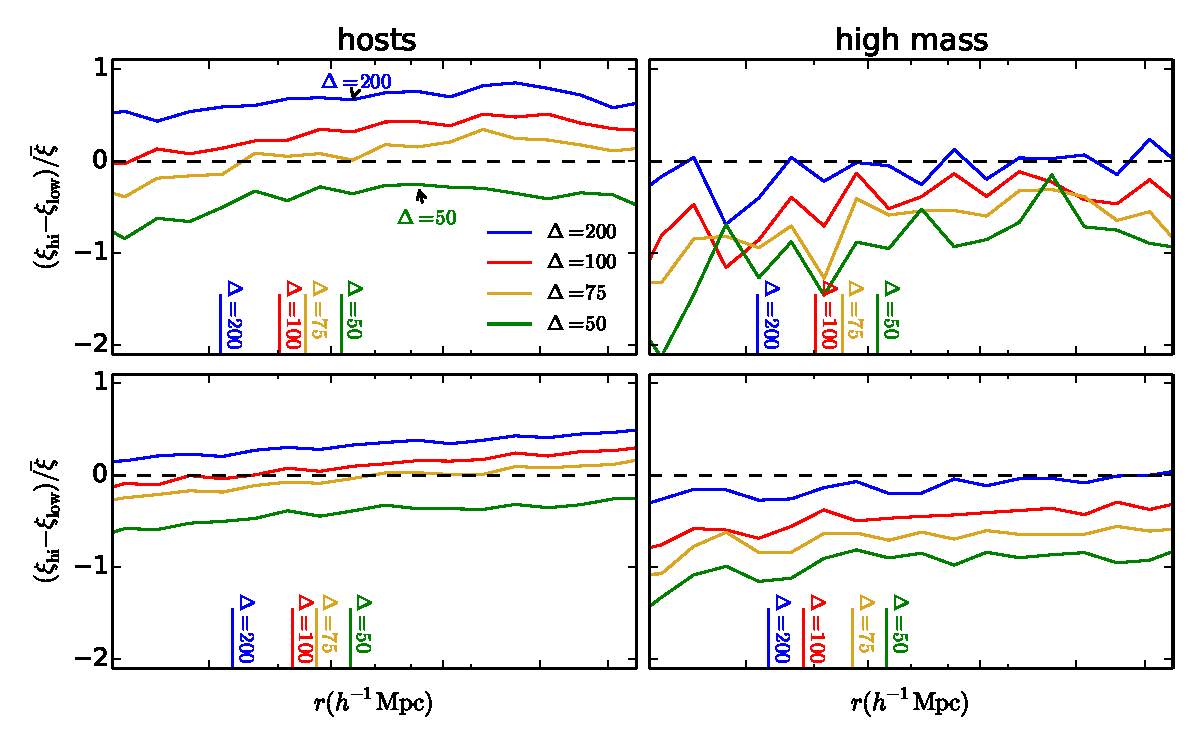
\includegraphics[width=.9\textwidth]{all_cfhilow_z00_hostsvhigh.pdf}
	\caption{The difference of the correlation function for only the top 20\% most concentrated halos and the bottom 20\% in concentration, normalized by the overall correlation function of the entire sample. The top row uses \simB \ data while the bottom row uses \simC \ data. The left column utilizes the ``mid mass'' cutoff, while the right column demonstrates the ``high mass'' cutoff. The dashed lines along the bottom denote the largest halo radius for a given value of the overdensity parameter}
	\label{fig:hvh_cfcompare}
\end{figure*}

\begin{figure*}
	\centering
	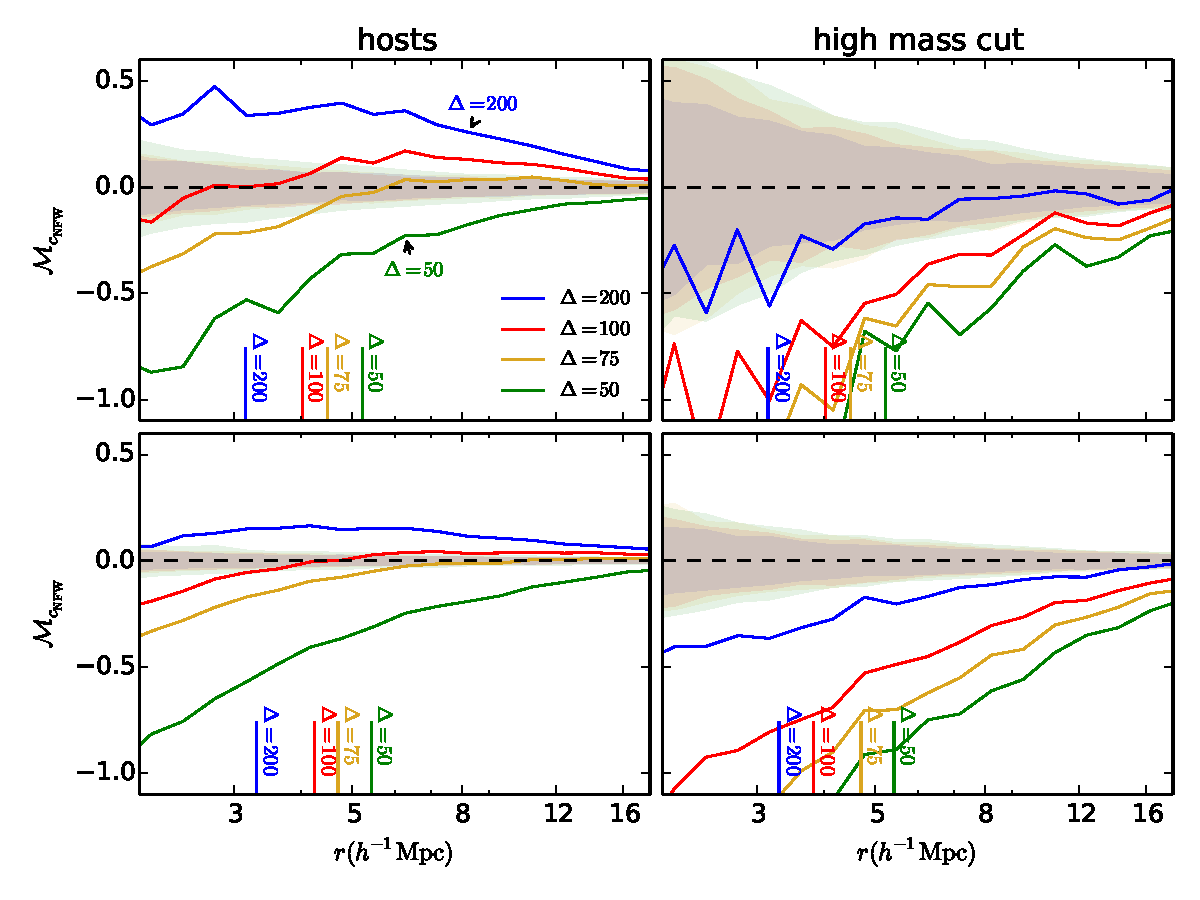
\includegraphics[width=.9\textwidth]{all_mcf_cnfw_z00_hostsvhigh.pdf}
	\caption{Comparison of the marked correlation function for the concentration defined according to the NFW profile between the ``mid mass'' cutoff (left column) and the ``high mass'' cutoff (right column). The top row uses \simB \ data while the bottom row uses \simC \ data. The shaded bands represent 2-sigma confidence regions generated by randomization of the marks. The dashed lines along the bottom denote the largest halo radius for a given value of the overdensity parameter.}
	\label{fig:hvh_mcf_cnfw}
\end{figure*}

\begin{figure*}
	\centering
	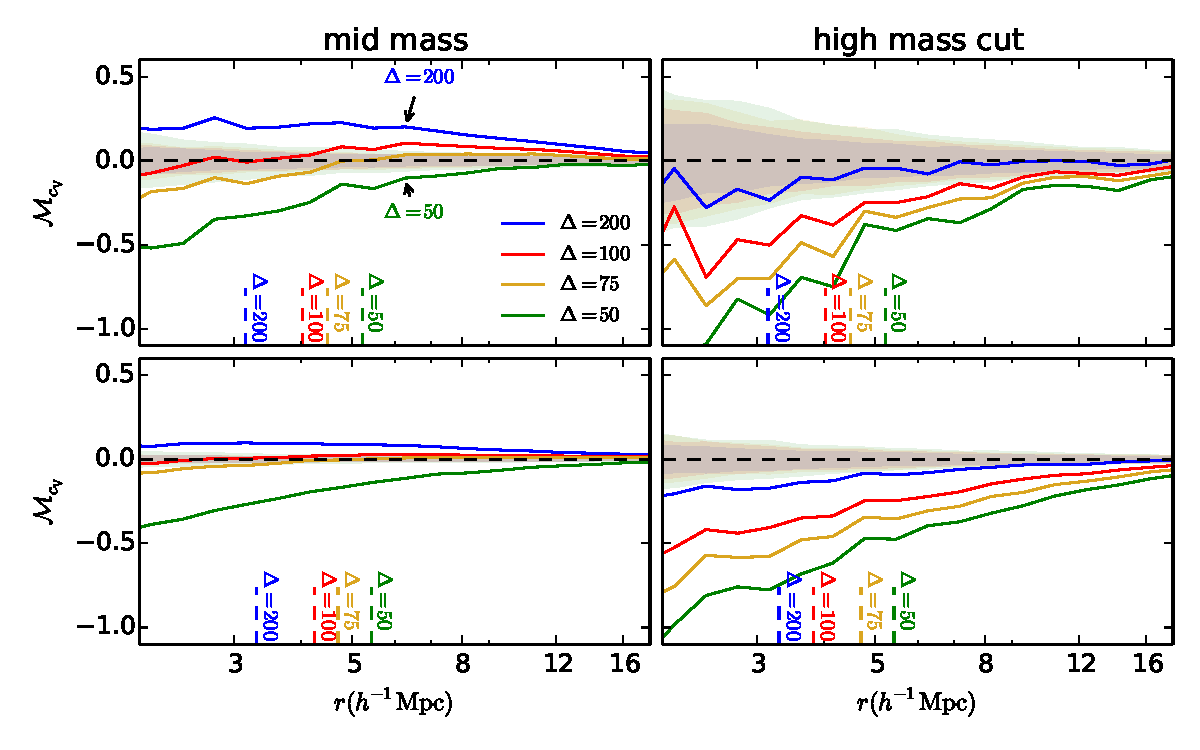
\includegraphics[width=.9\textwidth]{all_mcf_cV_z00_hostsvhigh.pdf}
	\caption{Comparison of the marked correlation function for the concentration defined according to the velocity ratio between the ``mid mass'' cutoff (left column) and the ``high mass'' cutoff (right column). The top row uses \simB \ data while the bottom row uses \simC \ data. The shaded bands represent 2-sigma confidence regions generated by randomization of the marks. The dashed lines along the bottom denote the largest halo radius for a given value of the overdensity parameter.}
	\label{fig:hvh_mcf_cV}
\end{figure*}

\begin{figure*}
	\centering
	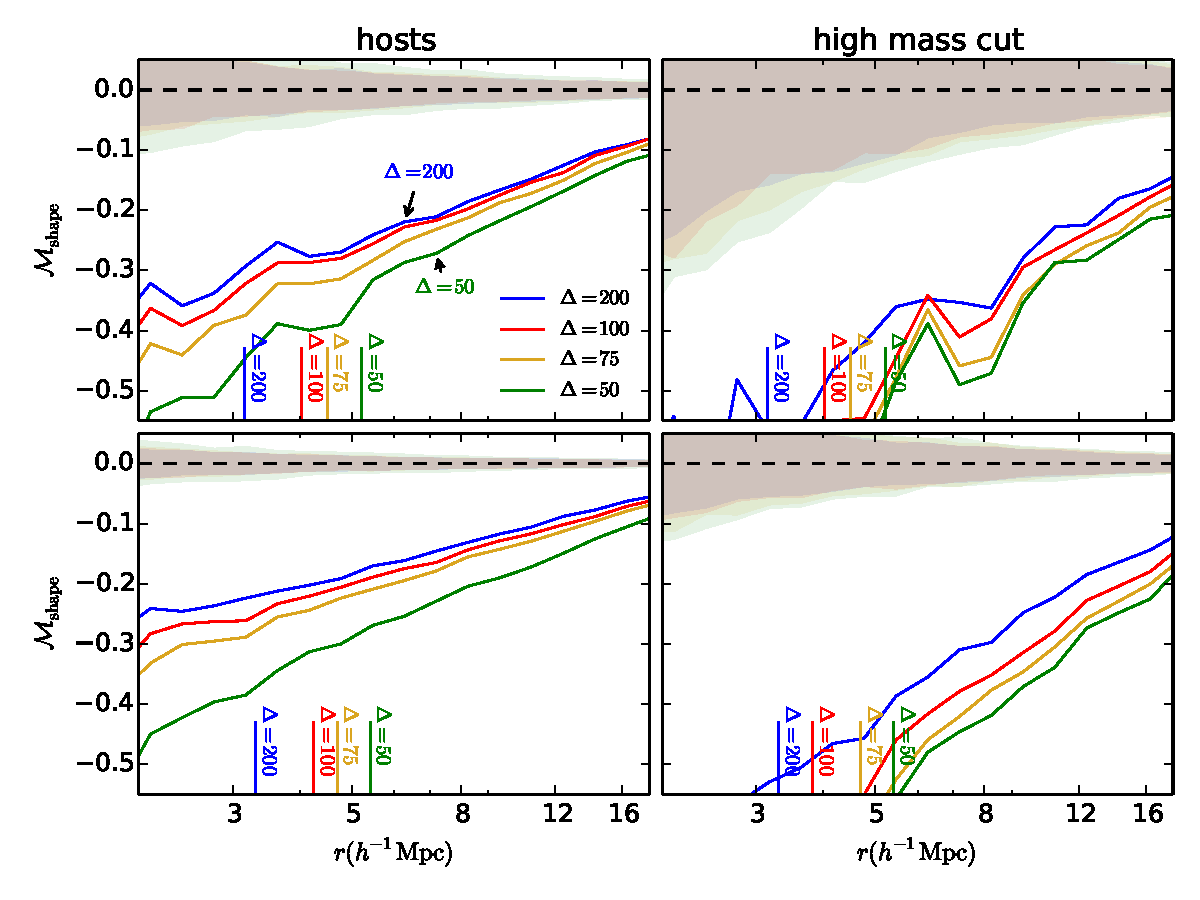
\includegraphics[width=.9\textwidth]{all_mcf_s_z00_hostsvhigh.pdf}
	\caption{Comparison of the marked correlation function for the shape of the halo between the ``mid mass'' cutoff (left column) and the ``high mass'' cutoff (right column). The top row uses \simB \ data while the bottom row uses \simC \ data. The shaded bands represent 2-sigma confidence regions generated by randomization of the marks. The dashed lines along the bottom denote the largest halo radius for a given value of the overdensity parameter.}
	\label{fig:hvh_mcf_s}
\end{figure*}

\begin{figure*}
	\centering
	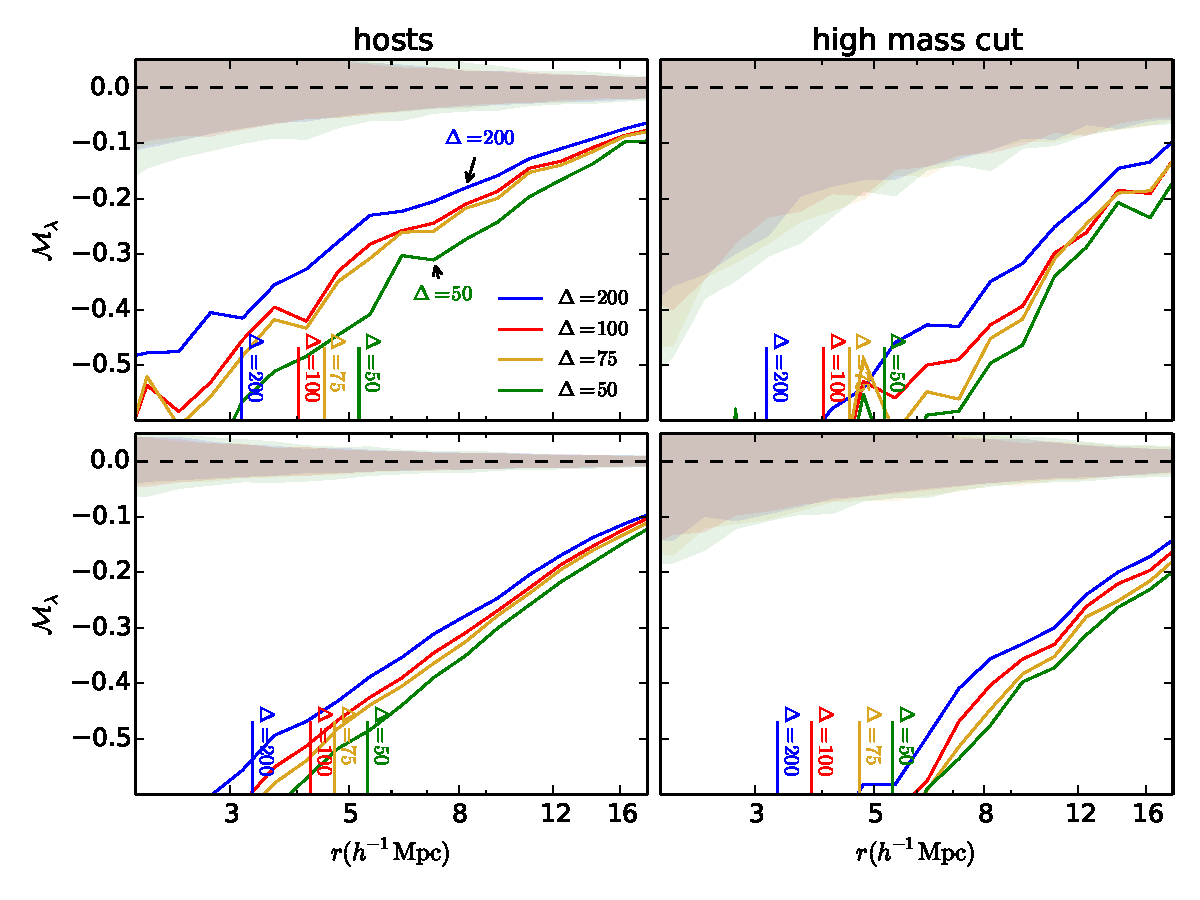
\includegraphics[width=.9\textwidth]{all_mcf_spin_z00_hostsvhigh.pdf}
	\caption{Comparison of the marked correlation function for the spin of the halo between the ``mid mass'' cutoff (left column) and the ``high mass'' cutoff (right column). The top row uses \simB \ data while the bottom row uses \simC \ data. The shaded bands represent 2-sigma confidence regions generated by randomization of the marks. The dashed lines along the bottom denote the largest halo radius for a given value of the overdensity parameter.}
	\label{fig:hvh_mcf_spin}
\end{figure*}

\begin{figure*}
	\centering
	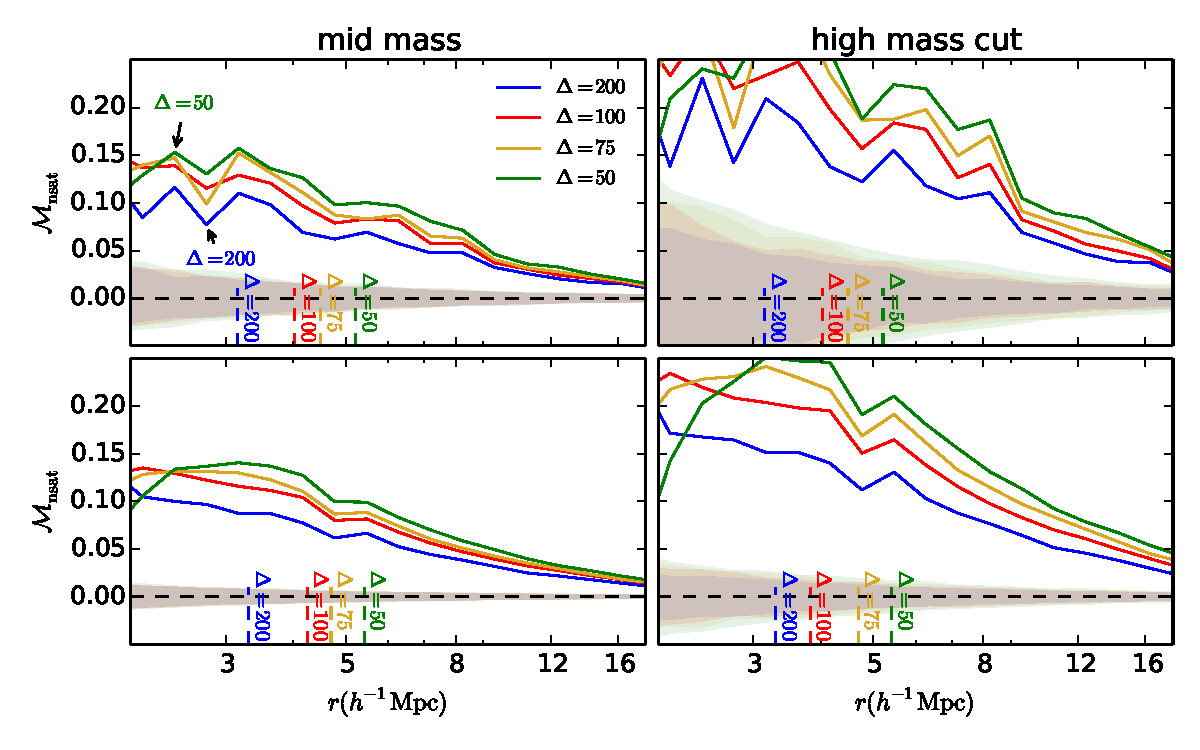
\includegraphics[width=.9\textwidth]{all_mcf_nsat_z00_hostsvhigh.pdf}
	\caption{Comparison of the marked correlation function for the satellite number between the ``mid mass'' cutoff (left column) and the ``high mass'' cutoff (right column). The top row uses \simB \ data while the bottom row uses \simC \ data. The shaded bands represent 2-sigma confidence regions generated by randomization of the marks. The dashed lines along the bottom denote the largest halo radius for a given value of the overdensity parameter.}
	\label{fig:hvh_mcf_nsat}
\end{figure*}

%----------------------
\section[]{Conclusions}
\label{section:conclusions}
%----------------------

We have looked at how to use CFs and MCFs in order to analyze the environmental effects upon the properties of the halo. We have suggested a method of removing the mass dependence that is not subject to the small number statistics at large halo masses. Taking our various tests, we then apply a change to the threshold density $\Delta$ in an attempt to remove the effect that environment has upon these properties. We come to the following conclusions from our simulation data.

\begin{itemize}
	\item Our halo redefinition method does not cause any substantial breakdown in the ROCKSTAR halo finding algorithm, though this may not be the case for every halo finding methodology. This is something that should be considered prior to utilization of this method, unless working directly from particle data. As our initial halo sizes and locations are determined through spherical overdensities, it cannot be assumed that starting from a FoF grouping and then determining values through particle data directly will produce identical results. Similarly, different cosmologies may remove environmental effects at different scales.

	\item When looking at the two-point correlation function, there appears to be a ``sweet spot'' that appears to remove environmental effects the most efficiently. Going beyond that seems to reintroduce environmental effects, possibly as an extreme side effect of halo exclusion.

	\item For our marked correlation functions we see that both proxies of concentration that we use as marks show significant removal of environmental effects at large scales for similar values of the overdensity parameter $\Delta$. In cases where one is only interested in the concentration of dark matter halos and large scales (or correspondingly small values of k), this method will allow you to compensate for bias that environment could introduce to calculations dependent upon the halo model. This may prove valuable for calculations such as that of the shear power spectrum calculated through weak lensing.

	\item The environmental effects on the shape of the host halo and the satellite number of the host halo cannot be removed regardless of the chosen redefinition of $\Delta$. We propose that this may be intrinsically tied to the nature of the filaments, whose effects cannot be removed by a simple redefinition of the halo radius.

	\item This method is definitively related to the mass of the halos that are being observed. Furthermore, it appears that the majority of the reduction in assembly bias is tied to the exclusion of halos from the catalog as a result of being subsumed into larger halos. This information does not seem to be contradictory; it can be intuitively understood that the region about the most massive halos will be different than the region around the least massive halos, leading to a different frequency at which halos are being excluded. It does however warrant that careful consideration be given to the sample of halos that are of interest.

	\item The selection of halo size is intrinsically related to the assembly bias and varies across scales. This might help to resolve contradictory results in the search for halo assembly bias in the literature.
\end{itemize}

This methodology, while certainly not perfect in accounting for assembly bias, may be of significance when applied to galaxy formation models and give insight into seemingly conflicting results. Provided that the properties of interest in a given model behave well under our redefinition, it will allow us to create better mock galaxy catalogs without resorting to more complicated models requiring halo formation histories - giving us another powerful tool to test observation against.

There remain possible uncertainties to study in the future. One possible area of follow-up is the matter of simulation cosmology, which is not explored in this text. It is possible that the choice of cosmology may change observed assembly bias as a function of the halo masses, something that our methodology should be capable of observing. Furthermore, we can determine if the choice of halo size that best reduces assembly bias is a function of the chosen cosmology. This may be of interest in attempting to determine signatures of assembly bias in observational samples in the future.

\section*{Acknowledgments}

We are grateful to many people.

%%\bibliographystyle{plainnat}
\bibliography{master}

\section*{Appendix}
\label{section:appendix_massres}

One natural question that might arise in the analysis of this work is the nature of the resulting assembly bias trends. Our focus in the main sections of this paper is on the nature of the assembly bias changing as a function of the mass cut chosen. Our conclusions include the fact that there is a strong mass dependence on halo assembly bias that must be accounted for seperately depending on the halos of interest in a study. However, while the existence of this trend is clear within our analysis, the determination that this is solely due to the masses of the halos included in our calculation is less clear upon closer inspection. One possibility that might be particularly concerning is the potential that the different simulations have created halos that have fundamentally different clustering and this is leading to the result that we are interpreting as a mass dependence on assembly bias. Thankfully, though our statistics become less meaningful to carry out this calculation, we can carry out a comparison using the same mass cut across two of our simulations, knowing that these will only contain well resolved halos.

While not addressed directly, Figure~\ref{fig:hvl_cfcompare} through Figure~\ref{fig:hvl_mcf_nsat} contain a demonstration of the result that we are seeking in the left column of panels. The lower left panels show various marks of interest for \simB \ using the ``mid mass'' cut on the data set. In comparison, the upper left panel contains the same marks of interest for the \simA \ using the same mass cut. In the latter, there are fewer halos in this mass cut range, as a result of the smaller simulation box size. However, we note that despite the additional noise in the data set, the behavior of the assembly bias measurement is nearly identical within tolerances accounting for differences between simulations and noise. This motivates our conclusion that the driver behind the behavior is the mass cut of the data sets rather than the resolution of the simulation.

\label{lastpage}

\end{document}
